\documentclass[a4paper,11pt]{scrreprt}
\usepackage[a4paper,margin=2.5cm]{geometry}
\usepackage{listings}
\usepackage{underscore}
\usepackage{graphicx}
\usepackage[utf8]{inputenc}
\usepackage[T1]{fontenc}
\usepackage[english]{babel}
\usepackage{booktabs,longtable,tabularx,array,multirow,enumitem,xcolor,float,caption}
\usepackage{needspace}
\usepackage{etoolbox}
\pretocmd{\section}{\Needspace{9\baselineskip}}{}{}
\usepackage{tikz}
\usetikzlibrary{arrows.meta,positioning,shapes.geometric,fit,calc,backgrounds}
\usepackage{hyperref}
\hypersetup{
    bookmarks=false,
    pdftitle={Software Requirements Specification - ICU Multimodal Patient Monitoring System},
    pdfauthor={Project Team},
    pdfsubject={Software Requirements Specification},
    pdfkeywords={SRS, ICU monitoring, computer vision, face and eye analysis, React, Node.js, MongoDB},
    colorlinks=true,
    linkcolor=blue,
    citecolor=black,
    filecolor=black,
    urlcolor=purple,
    linktoc=page
}%
\def\myversion{1.0 }
\date{}

% ---------- Fill these in (title page) ----------
\newcommand{\authorone}{[Student Name 1] ([Roll No.])}
\newcommand{\authortwo}{[Student Name 2] ([Roll No.])}
\newcommand{\supervisor}{[Supervisor Name]}
\newcommand{\supervisortitle}{[Designation, Department]}

% ---------- Requirement tables ----------
\setlist{itemsep=2pt,topsep=4pt}
\captionsetup{font=small,labelfont=bf}
\newenvironment{reqtable}[1]{%
  \small
  \begin{longtable}{@{}>{\ttfamily\footnotesize}p{2.55cm}>{\raggedright\arraybackslash}p{10.7cm}c@{}}
  \caption{#1}\\
  \toprule \textbf{ID} & \textbf{Requirement} & \textbf{Pri.}\\ \midrule
  \endfirsthead
  \toprule \textbf{ID} & \textbf{Requirement} & \textbf{Pri.}\\ \midrule
  \endhead
  \bottomrule
  \endfoot
}{%
  \end{longtable}\normalsize
}
\newcommand{\req}[3]{#1 & #2 & #3 \\ \midrule}
\newcommand{\code}[1]{\texttt{#1}}
\newcommand{\actor}[3]{\begin{scope}[shift={(#2)}]\draw[thick] (0,0.38) circle (0.13); \draw[thick] (0,0.25)--(0,-0.12) (-0.22,0.1)--(0.22,0.1) (0,-0.12)--(-0.16,-0.45) (0,-0.12)--(0.16,-0.45); \node[font=\scriptsize\bfseries, below, align=center] at (0,-0.45) {#3}; \coordinate (#1) at (0,0.05); \end{scope}}

\newenvironment{idtable}[1]{%
  \small
  \begin{longtable}{@{}>{\ttfamily\footnotesize}p{1.9cm}>{\raggedright\arraybackslash}p{13.2cm}@{}}
  \caption{#1}\\
  \toprule \textbf{ID} & \textbf{Statement}\\ \midrule
  \endfirsthead
  \toprule \textbf{ID} & \textbf{Statement}\\ \midrule
  \endhead
  \bottomrule
  \endfoot
}{%
  \end{longtable}\normalsize
}
\newcommand{\idr}[2]{#1 & #2 \\ \midrule}

% ---------- TikZ styles (match the black-header look of the template figures) ----------
\tikzset{
  blk/.style={rectangle, fill=black, text=white, font=\bfseries\small, align=center, minimum height=6mm, inner sep=3pt},
  gra/.style={rectangle, fill=gray!30, font=\small, align=center, minimum height=6mm, inner sep=3pt},
  grb/.style={rectangle, fill=gray!12, font=\small, align=center, minimum height=6mm, inner sep=3pt},
  box/.style={rectangle, rounded corners=3pt, draw=black, thick, align=center, font=\small, inner sep=4pt, fill=white},
  gbox/.style={rectangle, rounded corners=3pt, draw=black, thick, align=center, font=\small, inner sep=4pt, fill=gray!15},
  ell/.style={ellipse, draw=black, thick, align=center, font=\small\bfseries, inner sep=3pt, fill=white},
  uc/.style={ellipse, draw=black, thick, align=center, font=\scriptsize, inner sep=1pt, fill=white, minimum width=3.4cm, minimum height=0.9cm},
  store/.style={rectangle, draw=black, thick, align=center, font=\scriptsize, inner sep=3pt, fill=gray!15},
  arr/.style={-{Stealth[length=2.4mm]}, thick},
  darr/.style={{Stealth[length=2.4mm]}-{Stealth[length=2.4mm]}, thick},
  lbl/.style={font=\scriptsize\color{blue!45!black}, inner sep=1.5pt, fill=white, fill opacity=0.85, text opacity=1},
  note/.style={font=\scriptsize\itshape, align=center}
}
% A table-like column: black header + alternating grey rows
\newcommand{\stack}[5]{% name, position, width, header, comma-separated rows
  \node[blk, minimum width=#3, anchor=north west] (#1-h) at (#2) {#4};
  \foreach \r [count=\i] in {#5} {
    \ifodd\i \tikzset{curr/.style={gra}}\else \tikzset{curr/.style={grb}}\fi
    \node[curr, minimum width=#3, anchor=north west] (#1-\i) at ([yshift={-(\i-1)*6mm}]#1-h.south west) {\r};
  }
}

\begin{document}

\begin{flushright}
    \rule{16cm}{5pt}\vskip1cm
    \begin{bfseries}
        \Huge{SOFTWARE REQUIREMENTS\\ SPECIFICATION}\\
        \vspace{1.5cm}
        for\\
        \vspace{1.5cm}
        \huge{ICU MULTIMODAL PATIENT\\ MONITORING SYSTEM}\\
        \vspace{0.4cm}
        \Large{with Real-Time Face and Eye Behaviour Analysis}\\
        \vspace{1.5cm}
        \LARGE{Version \myversion}\\
        \vspace{1.5cm}
        \large
        Prepared by : 1. Harjot Singh 1024240039\\
        2. Pahul Singh 1024240103\\
        \vspace{1.5cm}
        Submitted to : Dr.Anushka \\ 
        Assistant Professor, CSED\\
        \vspace{1.5cm}
        \today\\
    \end{bfseries}
\end{flushright}

\tableofcontents
\listoffigures
\listoftables

\chapter{Introduction}

\section{Purpose}
Intensive Care Units (ICUs) depend on continuous observation of patients. Physiological monitors, periodic charting and manual assessment remain the primary sources of information, but visual cues such as facial expression, eye closure and gaze behaviour are rarely captured in a structured, reviewable form. The team has already built a Python computer-vision pipeline (the \emph{Face + Eye Pipeline}) that extracts such cues from a camera stream. At present its results are shown in a local OpenCV window and written to CSV/JSONL logs; the small FastAPI service in the same repository keeps only the latest values in memory, has no database, no authentication and no user interface for clinical staff.

This document is the Software Requirements Specification (SRS) for the \textbf{ICU Multimodal Patient Monitoring System}, Version 1.0: a web platform that connects the existing pipeline to a full-stack application (React + Vite, Node.js + Express, MongoDB Atlas) so that authorised users can view live face-and-eye observations, review history, receive configured event alerts and manage ICU patient records from one interface. The SRS defines what the system shall do and the limits within which it shall operate. It is the baseline for design, implementation, testing and acceptance.

The system is a \textbf{research and monitoring-support prototype}. It does not diagnose, does not recommend treatment and does not replace physiological measurement or clinical judgement.

\section{Document Conventions}\label{sec:conventions}
\begin{itemize}
  \item \textbf{Requirement identifiers} follow the pattern \code{FR-<MODULE>-nn} (functional), \code{CVI-nn} (changes required in the existing CV pipeline), \code{NFR-<CATEGORY>-nn} (non-functional), \code{DR-nn} (data), \code{IR-<TYPE>-nn} (interface), \code{C-nn} (constraint), \code{A-nn} (assumption), \code{BR-nn} (business rule) and \code{R-nn} (risk or known issue).
  \item \textbf{Keywords.} ``Shall'' marks a mandatory requirement, ``should'' a recommended one and ``may'' an optional one.
  \item \textbf{Priority} uses MoSCoW: \textbf{M} = Must have (needed for the core demonstration), \textbf{S} = Should have, \textbf{C} = Could have (only if time permits). Items that are deliberately excluded are listed in Section~\ref{sec:outofscope}.
  \item \textbf{Numeric targets} (latencies, timeouts, rates, retention periods) are initial design targets. They shall be confirmed with the supervisor and validated by testing before being quoted as achieved results.
  \item \textbf{Evidence about the CV pipeline.} Statements about the existing pipeline come from the project hand-off document, which is a static review of the public repository (branch \code{main}, commit \code{5405f41}, dated 2026-07-08). The pipeline has not been run end-to-end against the new platform; behaviour must be re-verified during integration (Phase 5 of the proposal).
\end{itemize}

\section{Intended Audience and Reading Suggestions}
This SRS is written for developers, the project supervisor and evaluators, testers, and any clinical or ethics adviser who reviews the project. It covers external, internal, functional and non-functional aspects of the system.
\begin{itemize}
  \item \textbf{Supervisor / evaluators:} read Chapters 1 and 2, then Appendix~\ref{app:trace} (traceability) and Section~\ref{sec:risks} (known issues).
  \item \textbf{Frontend developers:} Sections~\ref{sec:ui}, \ref{sec:features} (features 1--3 and 7--14) and Appendix~\ref{app:ui}.
  \item \textbf{Backend developers:} Sections~\ref{sec:features} (features 2--9), \ref{sec:cvi}, \ref{sec:api} and \ref{sec:data}.
  \item \textbf{CV / pipeline developers:} Sections~\ref{sec:cvi}, \ref{sec:payload} and \ref{sec:risks}.
  \item \textbf{Testers:} every requirement table in Chapter 3 and Chapter 4; each requirement is written to be testable.
\end{itemize}

\section{Project Scope}
The ICU Monitoring Platform creates a shared space for \textbf{administrators, doctors, nurses and family members} (Section~\ref{sec:users}) around one core capability: turning the output of the Face + Eye Pipeline into a persistent, access-controlled, reviewable record.

\medskip\noindent
A camera is placed at the bed. The Python pipeline detects and tracks one patient face, estimates facial Action Units (AUs), head pose, eye closure, PERCLOS and gaze, and computes heuristic indices (pain-related facial behaviour, fear, fatigue, agitation, tension, a respiratory-distress proxy and a global distress score) together with episode flags. It sends a feature payload (and, optionally, a live preview frame) over HTTPS to the application backend. The backend validates and stores the data in MongoDB Atlas and serves it to role-specific dashboards. Around this core, the platform provides patient and monitoring-session management, an alert centre, historical analytics and the administrative workspaces that appear in the supplied reference video (staffing, rooms, shifts, tasks and medication records).

\begin{figure}[h!]
\centering
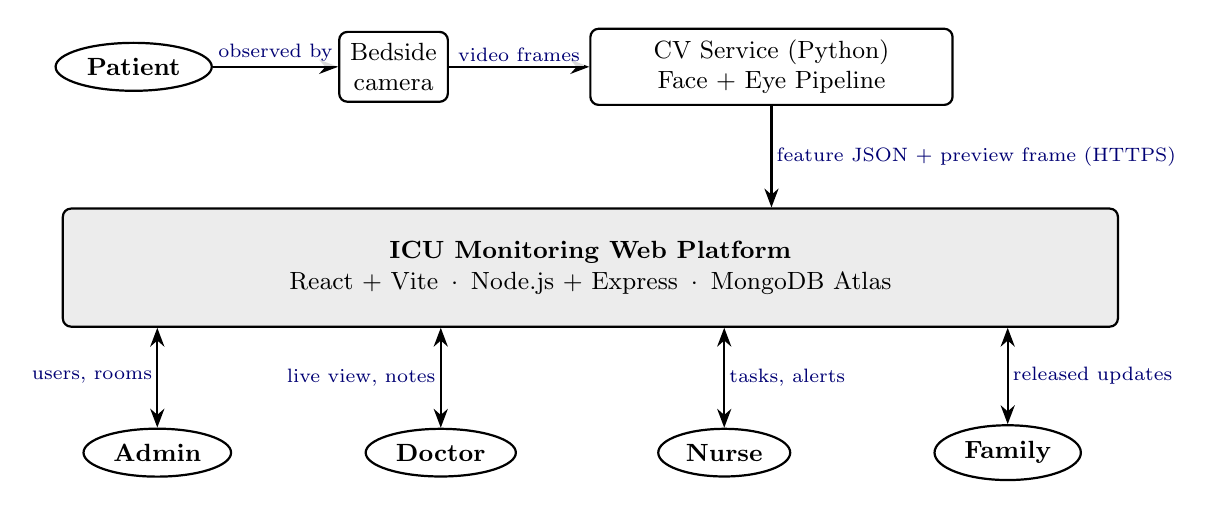
\begin{tikzpicture}[x=1cm,y=1cm]
  \node[ell] (pat) at (1.3,4.9) {Patient};
  \node[box] (cam) at (4.6,4.9) {Bedside\\camera};
  \node[box, minimum width=4.6cm] (cv) at (9.4,4.9) {CV Service (Python)\\Face + Eye Pipeline};
  \node[gbox, minimum width=13.4cm, minimum height=1.5cm] (plat) at (7.1,2.35) {\textbf{ICU Monitoring Web Platform}\\React + Vite \,$\cdot$\, Node.js + Express \,$\cdot$\, MongoDB Atlas};
  \node[ell] (adm) at (1.6,0) {Admin};
  \node[ell] (doc) at (5.2,0) {Doctor};
  \node[ell] (nur) at (8.8,0) {Nurse};
  \node[ell] (fam) at (12.4,0) {Family};
  \draw[arr] (pat) -- node[lbl,above]{observed by} (cam);
  \draw[arr] (cam) -- node[lbl,above]{video frames} (cv);
  \draw[arr] (cv.south) -- node[lbl,right]{feature JSON + preview frame (HTTPS)} (cv.south |- plat.north);
  \draw[darr] (adm) -- node[lbl,left]{users, rooms} (adm |- plat.south);
  \draw[darr] (doc) -- node[lbl,left]{live view, notes} (doc |- plat.south);
  \draw[darr] (nur) -- node[lbl,right]{tasks, alerts} (nur |- plat.south);
  \draw[darr] (fam) -- node[lbl,right]{released updates} (fam |- plat.south);
\end{tikzpicture}
\caption{System context: the existing CV pipeline feeds the new web platform, which serves four user roles.}
\label{fig:context}
\end{figure}

Figure~\ref{fig:context} gives the overview. The connections between the entities are interdependent: the camera feeds the pipeline, the pipeline feeds the platform, and every user role works only through the platform.

\subsection{In Scope}
\begin{itemize}
  \item Web application with landing page, workspace selection, role-based authentication and four workspaces (Admin, Doctor, Nurse, Family).
  \item Patient records, monitoring sessions and room/bed allocation.
  \item Versioned REST API for ingestion of face-and-eye feature payloads and preview frames from the Python service.
  \item Live (near-real-time) face-and-eye monitoring view with explicit stale, offline and missing-data states.
  \item Monitoring events, an alert centre with acknowledgement, and historical charts for each session.
  \item Administrative record keeping for care tasks, medication schedules, shifts and staff activity.
  \item Deployment on Vercel (frontend), Render (backend) and MongoDB Atlas (database); the CV service runs on a separate machine with the camera.
\end{itemize}

\subsection{Out of Scope}\label{sec:outofscope}
The reference video shows several capabilities that this version does \emph{not} implement. They shall not appear in the interface with invented data (BR-03, FR-LIVE-16).
\begin{itemize}
  \item Clinical diagnosis, treatment advice, automatic medication decisions or drug-interaction checking.
  \item Acquisition of physiological vitals (heart rate, SpO$_2$, blood pressure, core temperature) and the ``AI risk prediction'' widgets (e.g.\ sepsis probability), lab results and a seizure score.
  \item The posture (pose) and audio analysis modules (the posture module is separate in the repository).
  \item Equipment inventory, billing, and integration with hospital information systems (HL7, FHIR, EHR).
  \item Permanent video recording, native mobile applications and clinical validation of the CV indices.
\end{itemize}

\section{Project Objectives}
\begin{tabularx}{\textwidth}{@{}l>{\raggedright\arraybackslash}X@{}}
\toprule
\textbf{ID} & \textbf{Objective}\\ \midrule
O1 & Integrate the existing Face + Eye Pipeline through a documented, versioned HTTP contract, without re-implementing its algorithms.\\
O2 & Provide secure, server-enforced role-based access for administrators, doctors, nurses and family members.\\
O3 & Persist patients, monitoring sessions, feature snapshots, events and alerts in MongoDB Atlas.\\
O4 & Show live face-and-eye observations within the latency target of NFR-PERF-01, and represent missing, stale or unavailable data explicitly.\\
O5 & Convert pipeline episode flags into events and alerts that staff can review and acknowledge.\\
O6 & Provide historical charts and session summaries based on recorded observations only.\\
O7 & Support the operational ICU modules shown in the reference video (rooms, shifts, tasks, medication records) as administrative record keeping.\\
O8 & Deliver a responsive interface modelled on the supplied reference video.\\
O9 & Deploy frontend, backend and database to the chosen cloud services and connect them securely to the CV service.\\
O10 & Test the complete data flow and document the architecture, limitations and future work, without presenting heuristic scores as clinically validated.\\
\bottomrule
\end{tabularx}

\section{Definitions, Acronyms and Abbreviations}
\begin{longtable}{@{}>{\bfseries}p{3.1cm}p{12.4cm}@{}}
\toprule Term & Meaning\\ \midrule \endhead
AU & Facial Action Unit; here a continuous geometric score estimated from facial landmarks (15 AUs), not a validated FACS intensity.\\
Alert & A notification raised by the platform from an event or rule and shown in the alert centre until acknowledged.\\
Baseline & Per-patient reference values collected by the pipeline during an initial period (about 30 s) before personal deviations are used.\\
Behaviour state & Rule-based label from the pipeline: \code{alert}, \code{drowsy}, \code{eye_closed}, \code{fixation} or \code{scanning}.\\
CV Service & The Python Face + Eye Pipeline running on the machine with the camera.\\
EAR & Eye Aspect Ratio, used to estimate eye closure.\\
Episode / Event & A period during which a configured threshold persists (pain, agitation, fatigue, fear, eye closure). The pipeline calls it an \emph{episode}; the platform stores it as a \emph{monitoring event}.\\
Global distress & Weighted heuristic score from 0 to 100 combining the pain, fear, fatigue, agitation, tension and respiratory indices.\\
Heuristic index & A score computed by fixed rules from visual features; not a direct physiological or clinical measurement.\\
L2CS-Net & Pretrained neural network used by the pipeline for gaze yaw and pitch.\\
MediaPipe Face Mesh & Library used for face detection and 468-point landmark extraction.\\
PERCLOS & Percentage of eye closure over a rolling time window.\\
RBAC & Role-Based Access Control.\\
REST / JSON & Representational State Transfer API style; JavaScript Object Notation payloads.\\
JWT & JSON Web Token used for authentication.\\
SPA & Single-Page Application (the React frontend).\\
Session & A monitoring session: the period during which a CV Service streams data for one patient.\\
Snapshot & One stored feature payload (a time-stamped set of face-and-eye values).\\
Stale data & The latest snapshot is older than the configured freshness threshold.\\
TTL index & MongoDB index that automatically deletes documents after a set age.\\
\bottomrule
\end{longtable}

\section{References}
\begin{enumerate}[label={[\arabic*]}]
  \item Project Proposal, \emph{ICU Multimodal Patient Monitoring System with Real-Time Face and Eye Behaviour Analysis}.
  \item \emph{Face + Eye Pipeline --- Complete Technical Handoff} (\code{FACE_EYE_PIPELINE_HANDOFF.md}), prepared 2026-10-16.
  \item Source repository: \url{https://github.com/krishgakhar/2D_FaceAndEye_Pipline} (branch \code{main}, commit \code{5405f41}).
  \item Supplied ICU monitoring interface reference video (landing page, workspace selection, doctor, nurse and admin screens).
  \item ISO/IEC/IEEE 29148:2018, \emph{Systems and software engineering --- Life cycle processes --- Requirements engineering}; IEEE Std 830-1998, \emph{Recommended Practice for Software Requirements Specifications}.
  \item SRS template (Overleaf), \emph{Software Requirements Specification --- IICT Website}, used for the chapter structure of this document.
\end{enumerate}

\chapter{Overall Description}

\section{Product Perspective}
The platform is a new, self-contained web system that \emph{wraps} an existing component. It does not replace the Face + Eye Pipeline; it replaces the pipeline's temporary delivery path (local window, CSV/JSONL files and the in-memory FastAPI prototype exposing \code{/face}, \code{/posture} and \code{/fusion}) with a persistent, authenticated, multi-user service. Three layers cooperate (Figure~\ref{fig:arch}):

\begin{enumerate}
  \item \textbf{Frontend} --- React + Vite single-page application on Vercel.
  \item \textbf{Application backend} --- Node.js + Express REST API on Render, with MongoDB Atlas as database. The backend never executes the Python pipeline inside its own process.
  \item \textbf{CV Service} --- the existing Python pipeline on a machine that has the camera. It pushes validated payloads to the backend.
\end{enumerate}

\begin{figure}[h!]
\centering
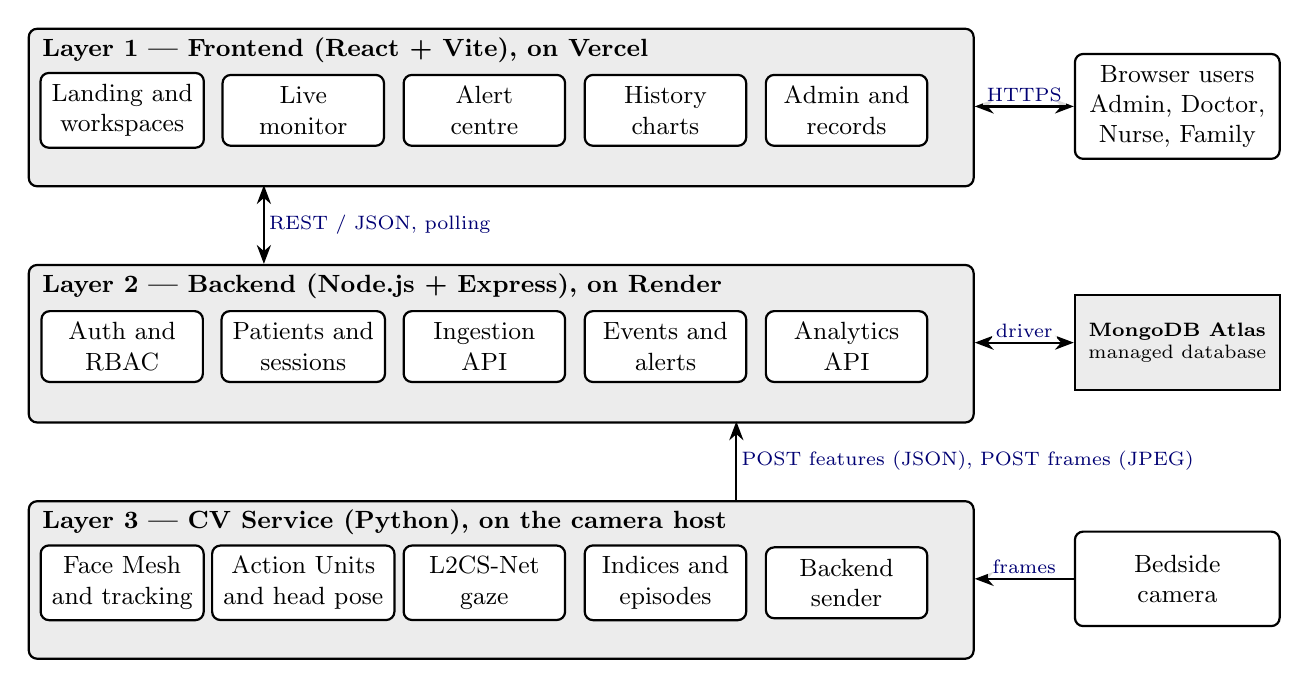
\begin{tikzpicture}[x=1cm,y=1cm, every node/.style={font=\scriptsize}]
  % layer frames
  \node[gbox, minimum width=12.0cm, minimum height=2.0cm, anchor=north west] (L1) at (0,7.4) {};
  \node[gbox, minimum width=12.0cm, minimum height=2.0cm, anchor=north west] (L2) at (0,4.4) {};
  \node[gbox, minimum width=12.0cm, minimum height=2.0cm, anchor=north west] (L3) at (0,1.4) {};
  \node[anchor=north west, font=\bfseries\small] at (L1.north west) {\,Layer 1 --- Frontend (React + Vite), on Vercel\,};
  \node[anchor=north west, font=\bfseries\small] at (L2.north west) {\,Layer 2 --- Backend (Node.js + Express), on Render\,};
  \node[anchor=north west, font=\bfseries\small] at (L3.north west) {\,Layer 3 --- CV Service (Python), on the camera host\,};
  % sub-boxes layer 1
  \foreach \x/\t in {1.2/Landing and\\workspaces, 3.5/Live\\monitor, 5.8/Alert\\centre, 8.1/History\\charts, 10.4/Admin and\\records}
    \node[box, minimum width=2.05cm, minimum height=0.9cm] at (\x,6.35) {\t};
  \foreach \x/\t in {1.2/Auth and\\RBAC, 3.5/Patients and\\sessions, 5.8/Ingestion\\API, 8.1/Events and\\alerts, 10.4/Analytics\\API}
    \node[box, minimum width=2.05cm, minimum height=0.9cm] at (\x,3.35) {\t};
  \foreach \x/\t in {1.2/Face Mesh\\and tracking, 3.5/Action Units\\and head pose, 5.8/L2CS-Net\\gaze, 8.1/Indices and\\episodes, 10.4/Backend\\sender}
    \node[box, minimum width=2.05cm, minimum height=0.9cm] at (\x,0.35) {\t};
  % side elements
  \node[box, minimum width=2.6cm, minimum height=1.2cm] (users) at (14.6,6.4) {Browser users\\Admin, Doctor,\\Nurse, Family};
  \node[store, minimum width=2.6cm, minimum height=1.2cm] (atlas) at (14.6,3.4) {\textbf{MongoDB Atlas}\\managed database};
  \node[box, minimum width=2.6cm, minimum height=1.2cm] (cam) at (14.6,0.4) {Bedside\\camera};
  \draw[darr] (L1.east |- users) -- node[lbl,above]{HTTPS} (users.west);
  \draw[darr] (L2.east |- atlas) -- node[lbl,above]{driver} (atlas.west);
  \draw[arr] (cam.west) -- node[lbl,above]{frames} (L3.east |- cam);
  % vertical flows between layers
  \draw[darr] (3.0,5.4) -- node[lbl,right]{REST / JSON, polling} (3.0,4.4);
  \draw[arr] (9.0,1.4) -- node[lbl,right]{POST features (JSON), POST frames (JPEG)} (9.0,2.4);
\end{tikzpicture}
\caption{Layered architecture and main data flow: camera $\rightarrow$ CV Service $\rightarrow$ backend $\rightarrow$ MongoDB Atlas $\rightarrow$ React dashboard.}
\label{fig:arch}
\end{figure}

\section{Stakeholders}\label{sec:stakeholders}
\begin{longtable}{@{}>{\bfseries\raggedright\arraybackslash}p{3.2cm}>{\raggedright\arraybackslash}p{4.6cm}>{\raggedright\arraybackslash}p{7.2cm}@{}}
\caption{Stakeholders and their concerns}\\
\toprule Stakeholder & Role & Interest and main concerns\\ \midrule \endfirsthead
\toprule Stakeholder & Role & Interest and main concerns\\ \midrule \endhead
\bottomrule \endfoot
Doctors (intensivists) & Primary users of the live monitor, alert centre and history. & Timely, understandable signals; avoiding alert fatigue; not over-interpreting heuristic scores.\\ \midrule
ICU nurses & Bedside users; acknowledge alerts, record tasks and medication administration. & Fast, low-effort screens during care; clear stale or offline indicators.\\ \midrule
ICU / hospital administrators & Manage users, rooms, staffing and system status. & Correct access control, audit trail, system availability.\\ \midrule
Patients & Subjects observed by the camera. & Privacy, dignity and consent; no unnecessary storage of video; minimum personal data.\\ \midrule
Family / guardians & Receive limited, released updates. & Understandable information without exposure of raw monitoring data.\\ \midrule
CV / ML developers & Own the Face + Eye Pipeline and its payload. & A stable, versioned contract; sender changes that do not stall the camera loop.\\ \midrule
Web and backend developers & Build and deploy the platform. & Clear API contract, testable requirements, reproducible deployment.\\ \midrule
Supervisor and evaluators & Assess the project. & Traceability, honest statement of limitations, evidence from testing.\\ \midrule
Ethics / clinical adviser & Approves any use with real patients or volunteers. & Consent, data minimisation, no unvalidated clinical claims.\\ \midrule
Cloud providers (Vercel, Render, MongoDB Atlas) & External services on which the system depends. & Plan limits, idle behaviour, credentials and network rules.\\
\end{longtable}

\section{User Classes and Characteristics}\label{sec:users}
The platform has four human user classes and one system actor (Figure~\ref{fig:users}). Staff accounts are created by an administrator; there is no public self-registration.

\begin{figure}[h!]
\centering
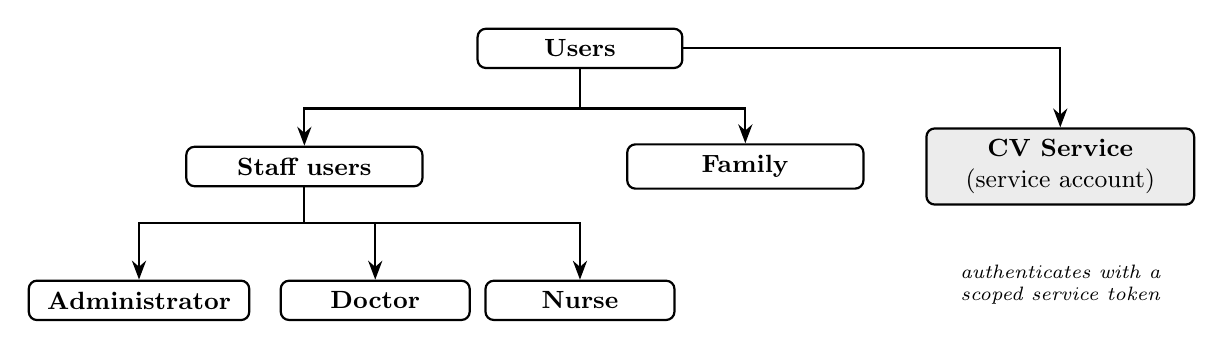
\begin{tikzpicture}[x=1cm,y=1cm]
  \node[box, minimum width=2.6cm] (users) at (6.5,3.2) {\textbf{Users}};
  \node[box, minimum width=3.0cm] (staff) at (3.0,1.7) {\textbf{Staff users}};
  \node[box, minimum width=3.0cm] (fam) at (8.6,1.7) {\textbf{Family}};
  \node[box, minimum width=3.4cm, fill=gray!15] (svc) at (12.6,1.7) {\textbf{CV Service}\\(service account)};
  \node[box, minimum width=2.8cm] (adm) at (0.9,0) {\textbf{Administrator}};
  \node[box, minimum width=2.4cm] (doc) at (3.9,0) {\textbf{Doctor}};
  \node[box, minimum width=2.4cm] (nur) at (6.5,0) {\textbf{Nurse}};
  \draw[arr] (users.south) -- ++(0,-0.5) -| (staff.north);
  \draw[arr] (users.south) -- ++(0,-0.5) -| (fam.north);
  \draw[arr] (users.east) -| (svc.north);
  \draw[arr] (staff.south) -- ++(0,-0.45) -| (adm.north);
  \draw[arr] (staff.south) -- ++(0,-0.45) -| (doc.north);
  \draw[arr] (staff.south) -- ++(0,-0.45) -| (nur.north);
  \node[note] at (12.6,0.2) {authenticates with a\\scoped service token};
\end{tikzpicture}
\caption{Types of users.}
\label{fig:users}
\end{figure}

\begin{longtable}{@{}>{\bfseries\raggedright\arraybackslash}p{2.6cm}>{\raggedright\arraybackslash}p{6.6cm}>{\raggedright\arraybackslash}p{5.8cm}@{}}
\caption{User classes}\\
\toprule Class & Description & Typical characteristics\\ \midrule \endfirsthead
\toprule Class & Description & Typical characteristics\\ \midrule \endhead
\bottomrule \endfoot
Administrator & Manages user accounts, rooms and beds, staffing views, system status and the audit log. Does not use the live clinical view. & Operations staff; works at a desk; needs overview screens and strict control of who can see what.\\ \midrule
Doctor & Reviews assigned patients, the live monitor, alerts and history; writes clinical notes; creates tasks and medication records; releases status notes to family. & High clinical expertise, limited time; mostly desktop or tablet; needs concise screens.\\ \midrule
Nurse & Checks in to a shift, watches assigned patients, acknowledges alerts, completes care tasks, records medication as given. & Frequent short interactions at the bedside, often on a tablet; needs large touch targets.\\ \midrule
Family member & Read-only access to a limited recovery summary of one linked patient. & Non-technical; may use a phone; must never see raw indices, video or other patients.\\ \midrule
CV Service & Non-human client that posts feature payloads, preview frames and heartbeats. & Runs unattended; authenticates with a revocable service token; has no access to user-facing data.\\
\end{longtable}

\noindent Table~\ref{tab:perm} fixes the permissions that the backend shall enforce (FR-WS-03).

\begin{table}[h!]
\centering\small
\caption{Role permission matrix. RW = read and write, R = read-only, (a) = assigned patients only, L = limited to released information of the linked patient, -- = no access.}
\label{tab:perm}
\begin{tabular}{@{}p{6.1cm}cccc@{}}
\toprule \textbf{Capability} & \textbf{Admin} & \textbf{Doctor} & \textbf{Nurse} & \textbf{Family}\\ \midrule
Sign in and select workspace & RW & RW & RW & RW\\
Create / edit patient records & RW & RW & R(a) & --\\
View patient list and details & R & R(a) & R(a) & L\\
Start / end monitoring session & -- & RW(a) & RW(a) & --\\
Live face-and-eye monitor & -- & R(a) & R(a) & --\\
Alert centre (view, acknowledge) & R & RW(a) & RW(a) & --\\
Patient-level history and charts & -- & R(a) & R(a) & --\\
Aggregate analytics (no identities) & R & -- & -- & --\\
Clinical notes & -- & RW(a) & R(a) & --\\
Care tasks & R & RW(a) & RW(a) & --\\
Medication schedule (record keeping) & -- & RW(a) & RW(a) & --\\
Shift check-in / check-out & -- & RW (own) & RW (own) & --\\
Rooms and bed allocation & RW & R & R & --\\
Staffing and staff activity & R & -- & -- & --\\
User management and credentials & RW & -- & -- & --\\
Audit log and system status & R & -- & -- & --\\
Messaging & RW & RW & RW & L\\
Released status updates & -- & RW(a) & -- & R\\
\bottomrule
\end{tabular}
\end{table}

\section{Product Functions}
The platform consists of the following functional modules (details in Chapter~3):
\begin{enumerate}[label=\arabic*.]
  \item Landing page, authentication and workspace selection.
  \item Patient and monitoring-session management.
  \item CV payload ingestion (features, heartbeat and preview frames).
  \item Live face-and-eye monitoring.
  \item Monitoring events and the alert centre.
  \item Historical analytics.
  \item Doctor, nurse, administrator and family workspaces, including rooms, shifts, tasks, medication records and messaging.
  \item Audit logging and system status.
\end{enumerate}

\begin{figure}[h!]
\centering
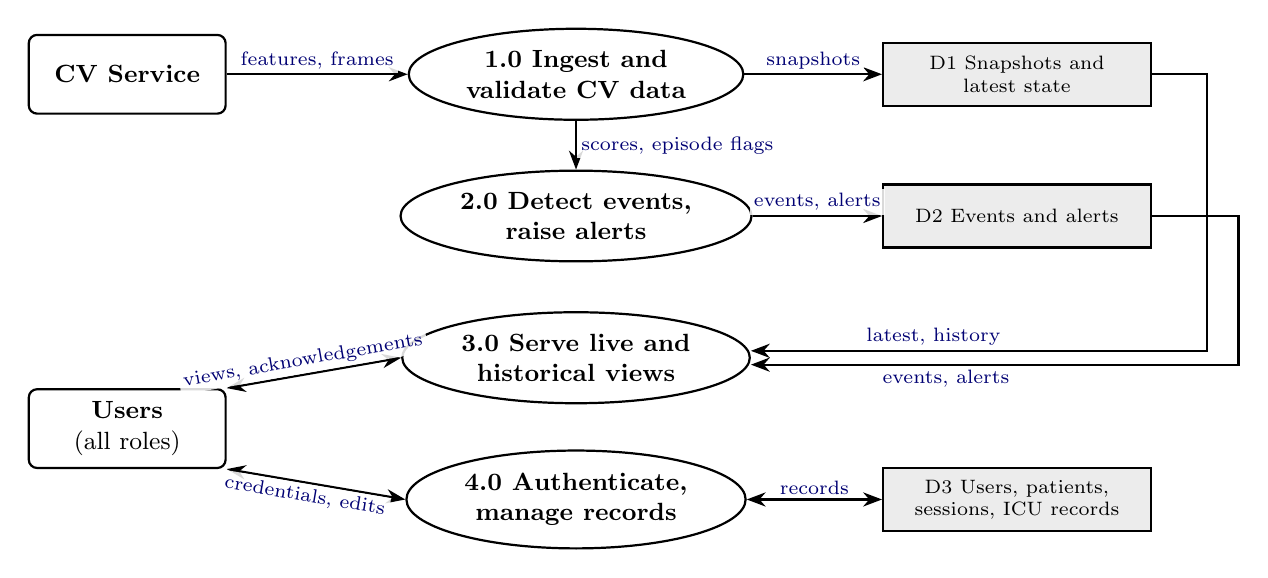
\begin{tikzpicture}[x=1cm,y=1cm, every node/.style={font=\scriptsize}]
  \node[box, minimum width=2.5cm, minimum height=1.0cm] (cv) at (1.3,5.4) {\textbf{CV Service}};
  \node[box, minimum width=2.5cm, minimum height=1.0cm] (usr) at (1.3,0.9) {\textbf{Users}\\(all roles)};
  \node[ell, minimum width=3.4cm, minimum height=1.1cm] (p1) at (7.0,5.4) {1.0 Ingest and\\validate CV data};
  \node[ell, minimum width=3.4cm, minimum height=1.1cm] (p2) at (7.0,3.6) {2.0 Detect events,\\raise alerts};
  \node[ell, minimum width=3.4cm, minimum height=1.1cm] (p3) at (7.0,1.8) {3.0 Serve live and\\historical views};
  \node[ell, minimum width=3.4cm, minimum height=1.1cm] (p4) at (7.0,0) {4.0 Authenticate,\\manage records};
  \node[store, minimum width=3.4cm, minimum height=0.8cm] (d1) at (12.6,5.4) {D1  Snapshots and\\latest state};
  \node[store, minimum width=3.4cm, minimum height=0.8cm] (d2) at (12.6,3.6) {D2  Events and alerts};
  \node[store, minimum width=3.4cm, minimum height=0.8cm] (d3) at (12.6,0) {D3  Users, patients,\\sessions, ICU records};
  \draw[arr] (cv) -- node[lbl,above]{features, frames} (p1);
  \draw[arr] (p1) -- node[lbl,above]{snapshots} (d1);
  \draw[arr] (p1) -- node[lbl,right]{scores, episode flags} (p2);
  \draw[arr] (p2) -- node[lbl,above]{events, alerts} (d2);
  \draw[arr] (d1.east) -- ++(0.7,0) |- node[lbl,above,pos=0.8]{latest, history} ([yshift=2.5pt]p3.east);
  \draw[arr] (d2.east) -- ++(1.1,0) |- node[lbl,below,pos=0.8]{events, alerts} ([yshift=-2.5pt]p3.east);
  \draw[darr] (usr.north east) -- node[lbl,above,sloped,pos=0.45]{views, acknowledgements} (p3.west);
  \draw[darr] (usr.south east) -- node[lbl,below,sloped,pos=0.45]{credentials, edits} (p4.west);
  \draw[darr] (p4) -- node[lbl,above]{records} (d3);
\end{tikzpicture}
\caption{Data flow diagram (Level 1).}
\label{fig:dfd}
\end{figure}

\begin{figure}[h!]
\centering
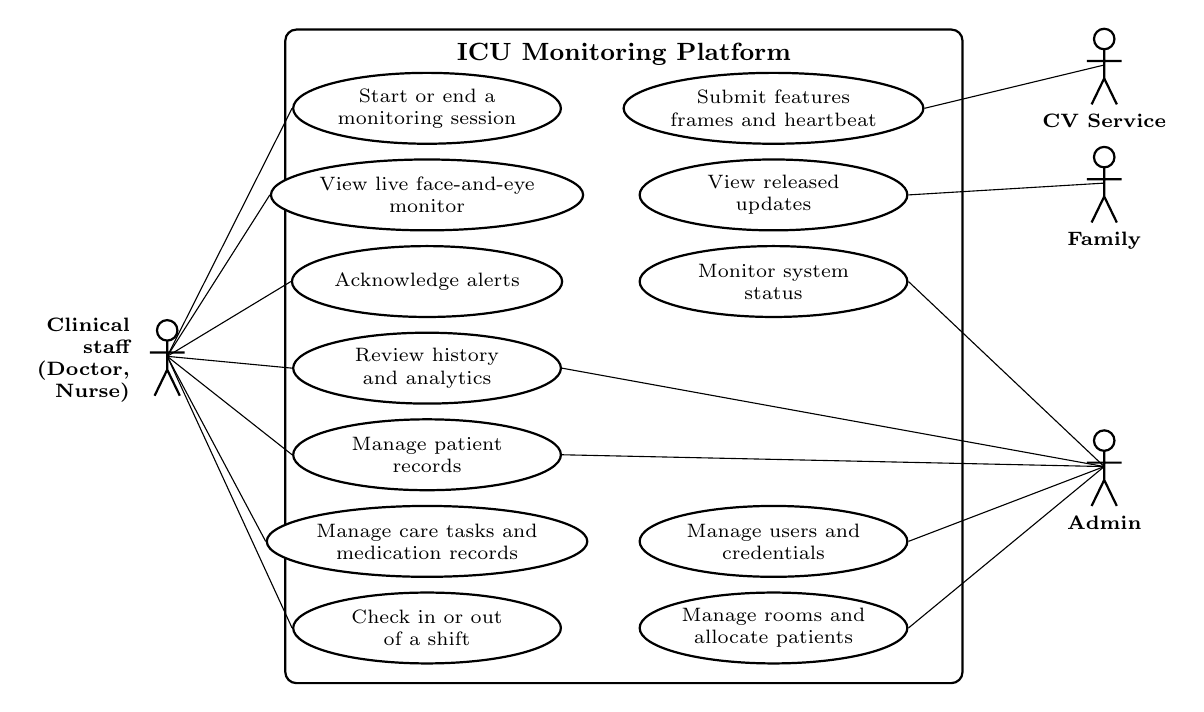
\begin{tikzpicture}[x=1cm,y=1cm]
  \draw[thick, rounded corners=4pt] (3.0,-1.1) rectangle (11.6,7.2);
  \node[font=\small\bfseries, anchor=north] at (7.3,7.15) {ICU Monitoring Platform};
  \foreach \y/\t [count=\i] in {6.2/Start or end a\\monitoring session, 5.1/View live face-and-eye\\monitor, 4.0/Acknowledge alerts, 2.9/Review history\\and analytics, 1.8/Manage patient\\records, 0.7/Manage care tasks and\\medication records, -0.4/Check in or out\\of a shift}
    \node[uc] (a\i) at (4.8,\y) {\t};
  \foreach \y/\t [count=\i] in {6.2/Submit features\\frames and heartbeat, 5.1/View released\\updates, 4.0/Monitor system\\status, 0.7/Manage users and\\credentials, -0.4/Manage rooms and\\allocate patients}
    \node[uc] (b\i) at (9.2,\y) {\t};
  \actor{clin}{1.5,3.0}{}
  \node[font=\scriptsize\bfseries, align=right, anchor=east] at (1.15,3.0) {Clinical\\staff\\(Doctor,\\Nurse)};
  \actor{adm}{13.4,1.6}{Admin}
  \actor{fam}{13.4,5.2}{Family}
  \actor{svc}{13.4,6.7}{CV Service}
  \foreach \i in {1,...,7} \draw[thin] (clin) -- (a\i.west);
  \draw[thin] (svc) -- (b1.east);
  \draw[thin] (fam) -- (b2.east);
  \draw[thin] (adm) -- (b3.east);
  \draw[thin] (adm) -- (b4.east);
  \draw[thin] (adm) -- (b5.east);
  \draw[thin] (adm) -- (a4.east);
  \draw[thin] (adm) -- (a5.east);
\end{tikzpicture}
\caption{Use-case diagram. Every human actor authenticates first (FR-AUTH); this is omitted for clarity. Doctor-only and nurse-only restrictions follow Table~\ref{tab:perm}.}
\label{fig:usecase}
\end{figure}

\section{Operating Environment}
\begin{itemize}
  \item \textbf{Client:} current versions of Chrome, Edge, Firefox and Safari on desktop, tablet and phone (viewport width from 360 px to 1920 px). No plug-ins are required.
  \item \textbf{Application backend:} Node.js (an active LTS release, fixed in \code{package.json}) with Express, hosted on Render.
  \item \textbf{Database:} MongoDB Atlas managed cluster.
  \item \textbf{CV Service:} Python 3.10 (as recommended in the repository README) on Windows or Linux, with a webcam or RGB camera, MediaPipe, OpenCV, PyTorch and the local weights file \code{models/L2CSNet_gaze360.pkl} (about 95.8 MB). A CUDA GPU is optional; a Jetson build uses \code{requirements/jetson.txt}.
  \item \textbf{Network:} the CV Service host needs outbound HTTPS access to the backend. No inbound connection to the CV host is required.
\end{itemize}

\section{Design and Implementation Constraints}\label{sec:constraints}
\begin{idtable}{Constraints}
\idr{C-01}{The frontend shall use React with Vite, the backend Node.js with Express, the database MongoDB Atlas; hosting shall use Vercel (frontend) and Render (backend). Source control uses Git and GitHub.}
\idr{C-02}{The Python pipeline shall remain a separate process. The Node.js backend shall not execute it in-process; they communicate only through the HTTP contract of Section~\ref{sec:api}.}
\idr{C-03}{A cloud-hosted website cannot reach a camera attached to a developer machine. The CV Service must therefore run where the camera is and push data to the cloud API.}
\idr{C-04}{The pipeline needs PyTorch, MediaPipe and a 95.8 MB weights file, and ideally a GPU. It shall not be assumed to fit the free tiers of Vercel or Render; the hosting decision for the CV Service is deferred (Appendix~\ref{app:open}).}
\idr{C-05}{The current sender posts feature payloads synchronously with a 1 s timeout from inside the camera loop. A slow backend therefore stalls inference; the ingestion endpoint must answer quickly (NFR-PERF-02) and the sender must be changed (CVI-03).}
\idr{C-06}{Preview frames are sent by a daemon thread that keeps only the latest frame with a 0.2 s timeout. Streaming is best-effort and lossy; it is a live preview, not an archive.}
\idr{C-07}{The pipeline scores one tracked face per camera. One CV instance therefore monitors one patient at a time, although MediaPipe may detect up to four faces.}
\idr{C-08}{All indices, behaviour states, severity bands and episodes are heuristics with software-defined thresholds. They are not clinically validated and shall be described as such in the interface and documents.}
\idr{C-09}{In the current code path gaze yaw and pitch are in radians. The contract shall state units explicitly; the interface converts to degrees for display.}
\idr{C-10}{The payload now sent to the backend is a subset of the data computed by the pipeline (no AUs, head-pose angles, PERCLOS, mean/max gaze speed or baseline flag). Displaying them requires a deliberate payload extension (CVI-02).}
\idr{C-11}{The current pipeline emits a payload only while a face is tracked and sends no heartbeat. Without a heartbeat the platform cannot distinguish ``no face in view'' from ``CV Service stopped'' (CVI-06).}
\idr{C-12}{Hosting plans may spin down idle services and limit database storage. Data volume shall be controlled by rate limiting, down-sampled history and TTL expiry (FR-ING-05, DR-05).}
\idr{C-13}{Patient data shall be limited to the minimum needed for the project, and camera frames shall not be stored permanently by default (NFR-PRV-01, NFR-PRV-02).}
\end{idtable}

\section{Assumptions and Dependencies}\label{sec:assumptions}
\begin{idtable}{Assumptions and dependencies}
\idr{A-01}{The pipeline behaviour described here matches the audited repository state (commit \code{5405f41}). Any divergence found during integration is recorded and this SRS is updated.}
\idr{A-02}{A monitoring session is bound to one patient. The \code{patient_id} sent by the CV Service (default \code{P001}) is mapped to a platform patient record by the person who starts the session.}
\idr{A-03}{The pipeline baseline period (about 30 s from start or after reset) is assumed to show a neutral face. This is an operating assumption, not something the system can verify.}
\idr{A-04}{The CV host and the backend have reasonably synchronised clocks. The backend stores both the capture time and its own receive time and uses the receive time for ordering.}
\idr{A-05}{The pipeline sender will be modified as specified in Section~\ref{sec:cvi}. Until then it will not work with the new API: it is disabled by default (\code{ENABLE_BACKEND = False}) and its routes differ from the contract.}
\idr{A-06}{Vercel, Render and MongoDB Atlas remain available under the plan selected for the project.}
\idr{A-07}{Testing uses volunteers, recorded or synthetic data. Use with real patients requires prior ethics approval and consent.}
\end{idtable}

\section{User Interface Design}\label{sec:ui}
The interface is modelled on the supplied reference video: a clean light theme with a blue accent, a public landing page, a ``Select Your Workspace'' page, one login portal per role, and a left-hand navigation rail inside each workspace. Appendix~\ref{app:ui} reproduces the reference screens. Table~\ref{tab:screens} lists the screens to be built.

\begin{figure}[h!]
\centering
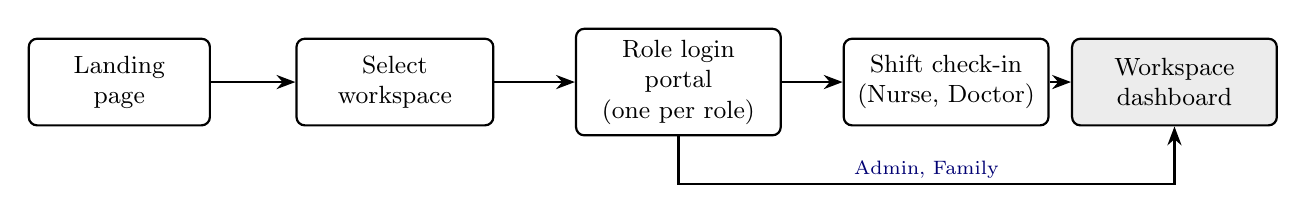
\begin{tikzpicture}[x=1cm,y=1cm]
  \node[box, minimum width=2.3cm, minimum height=1.1cm] (land) at (1.2,1.6) {Landing\\page};
  \node[box, minimum width=2.5cm, minimum height=1.1cm] (ws) at (4.7,1.6) {Select\\workspace};
  \node[box, minimum width=2.6cm, minimum height=1.2cm] (login) at (8.3,1.6) {Role login\\portal\\(one per role)};
  \node[box, minimum width=2.6cm, minimum height=1.1cm] (shift) at (11.7,1.6) {Shift check-in\\(Nurse, Doctor)};
  \node[box, minimum width=2.6cm, minimum height=1.1cm, fill=gray!15] (dash) at (14.6,1.6) {Workspace\\dashboard};
  \draw[arr] (land) -- (ws);
  \draw[arr] (ws) -- (login);
  \draw[arr] (login) -- (shift);
  \draw[arr] (shift) -- (dash);
  \draw[arr] (login.south) -- ++(0,-0.6) -| node[lbl,above,pos=0.25]{Admin, Family} (dash.south);
\end{tikzpicture}
\caption{Entry flow shared by all workspaces.}
\label{fig:entry}
\end{figure}

\begin{figure}[h!]
\centering
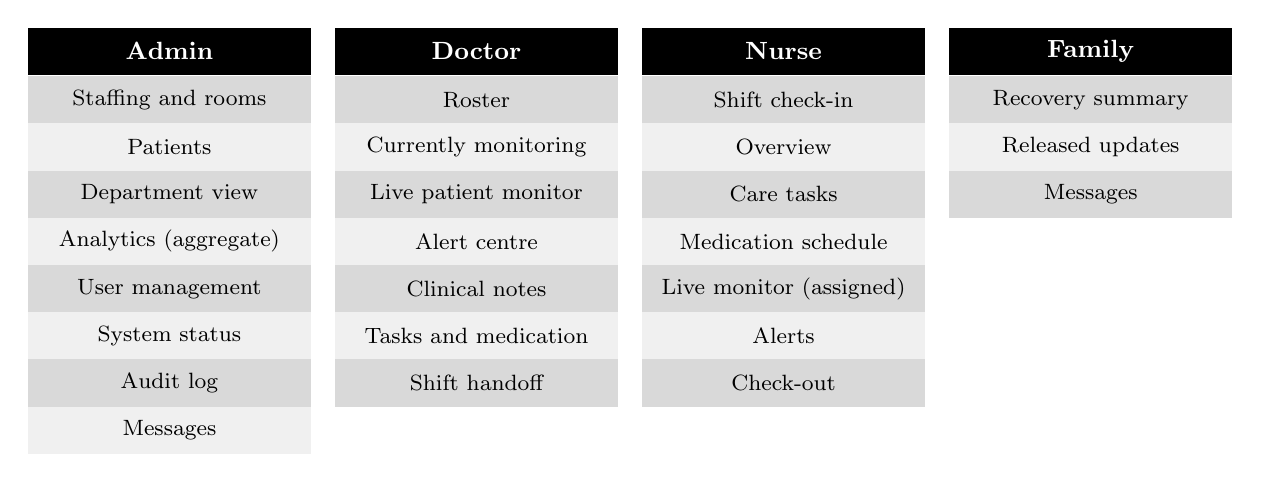
\begin{tikzpicture}[x=1cm,y=1cm]
  \begin{scope}[gra/.append style={font=\footnotesize}, grb/.append style={font=\footnotesize}]
  \stack{a}{0,0}{3.6cm}{Admin}{Staffing and rooms,Patients,Department view,Analytics (aggregate),User management,System status,Audit log,Messages}
  \stack{d}{3.9,0}{3.6cm}{Doctor}{Roster,Currently monitoring,Live patient monitor,Alert centre,Clinical notes,Tasks and medication,Shift handoff}
  \stack{n}{7.8,0}{3.6cm}{Nurse}{Shift check-in,Overview,Care tasks,Medication schedule,Live monitor (assigned),Alerts,Check-out}
  \stack{f}{11.7,0}{3.6cm}{Family}{Recovery summary,Released updates,Messages}
  \end{scope}
\end{tikzpicture}
\caption{Workspace activities by role.}
\label{fig:workspaces}
\end{figure}

\begin{longtable}{@{}>{\raggedright\arraybackslash}p{4.3cm}>{\raggedright\arraybackslash}p{8.2cm}>{\raggedright\arraybackslash}p{2.5cm}@{}}
\caption{Screen inventory derived from the reference video}\label{tab:screens}\\
\toprule Screen & Main content & Features\\ \midrule \endfirsthead
\toprule Screen & Main content & Features\\ \midrule \endhead
\bottomrule \endfoot
Landing page & Hero text, platform / how-it-works / safety sections, sign-in and request-access buttons, prototype disclaimer. & F1\\ \midrule
Select Your Workspace & Four tiles: Admin (System Ops), Doctor (Clinical Rounds), Nurse (Bedside Care), Family (My Recovery). & F3\\ \midrule
Role login portals & Admin Portal, Doctor Portal, Nurse Station: ID or e-mail, password with show toggle, sign-in button, forgot-credentials link. & F2\\ \midrule
Start of shift dialog & Nurse name, shift selector (e.g.\ Morning 07:00--15:00), check-in button. & F11\\ \midrule
Doctor dashboard & Header with shift status, emergency call and request handoff; active roster; ``currently monitoring'' panel with distress score; alert centre. & F10, F8\\ \midrule
Live Patient Monitor & Patient roster, distress score and alert level, Face \& Eye panel with preview and values, freshness indicator. Posture and audio panels are not built. & F7\\ \midrule
Nurse overview, care tasks, medication schedule & Assigned beds, pending medication, tasks due, last check; task list; scheduled medication with ``Given'' status. & F11\\ \midrule
Admin dashboard & Tabs for staffing, patients, department, analytics, user management, credentials and messages; floor and room management with allocate, deallocate and set-critical; alerts; active doctors; nurse activity dialog. & F12, F14\\ \midrule
Messages & Contact list and thread view, including system messages for shift check-in and check-out. & F14\\ \midrule
Family view & Read-only recovery summary of the linked patient. & F13\\
\end{longtable}

\chapter{System Features}
The ICU Monitoring Platform is a monitoring-support and record-keeping web system. Its main value is to turn the output of the Face + Eye Pipeline into stored, access-controlled and reviewable information; every other feature supports that flow.

\section{Description and Priority}\label{sec:features}
The features are listed from highest to lowest priority. All \textbf{Must} features are needed for the core demonstration; \textbf{Should} and \textbf{Could} features follow the reference video and are built if time allows.

\begin{longtable}{@{}c>{\raggedright\arraybackslash}p{4.6cm}l>{\raggedright\arraybackslash}p{4.3cm}>{\raggedright\arraybackslash}p{2.4cm}@{}}
\caption{Feature list, module codes and priorities}\label{tab:features}\\
\toprule \textbf{No.} & \textbf{Feature} & \textbf{Module} & \textbf{Reference} & \textbf{Priority}\\ \midrule \endfirsthead
\toprule \textbf{No.} & \textbf{Feature} & \textbf{Module} & \textbf{Reference} & \textbf{Priority}\\ \midrule \endhead
\bottomrule \endfoot
F6 & CV payload ingestion & ING & Proposal \S9; hand-off \S9 & Must\\
F7 & Live face-and-eye monitoring & LIVE & Live Patient Monitor screen & Must\\
F2 & Authentication & AUTH & Role login portals & Must\\
F3 & Workspace selection and access control & WS & Select Your Workspace & Must\\
F4 & Patient management & PAT & Roster, patient cards & Must\\
F5 & Monitoring-session management & SESS & Proposal \S10 & Must\\
F8 & Monitoring events and alert centre & EVT & Alert Center & Must\\
F9 & Historical analytics & HIST & Proposal \S8.7 & Must\\
F10 & Doctor workspace & DOC & Doctor dashboard & Should\\
F11 & Nurse workspace & NUR & Nurse overview, tasks, medication & Should\\
F12 & Administrator workspace & ADM & Admin dashboard & Should\\
F1 & Public landing page & LAND & Landing page & Should\\
F15 & Audit logging & AUD & Proposal \S12 & Should\\
F13 & Family workspace & FAM & My Recovery & Could\\
F14 & Messaging, emergency call, handoff & MSG & Messages, header buttons & Could\\
\end{longtable}

\section{Feature 1: Public Landing Page}
The landing page introduces the platform to visitors and routes them to sign-in. It describes the system honestly as a research prototype.
\begin{reqtable}{Landing page requirements}
\req{FR-LAND-01}{The system shall provide a public landing page that explains the platform's purpose and main capabilities and links to sign-in and workspace selection.}{S}
\req{FR-LAND-02}{The landing page shall state that the system is a research and monitoring-support prototype and not a diagnostic or treatment device.}{M}
\req{FR-LAND-03}{Any illustrative patient card on the landing page shall be labelled as sample data; it shall not appear as a live feed.}{M}
\req{FR-LAND-04}{The landing page shall not claim regulatory or security certifications (for example HIPAA or SOC~2) that the project has not obtained.}{M}
\end{reqtable}

\section{Feature 2: Authentication}
Only registered users can enter the system. Accounts are created by an administrator, and the CV Service has its own credential.
\begin{reqtable}{Authentication requirements}
\req{FR-AUTH-01}{The system shall let a registered user sign in with an e-mail or staff ID and a password and sign out.}{M}
\req{FR-AUTH-02}{Passwords shall be stored only as salted hashes produced by an adaptive algorithm (bcrypt or Argon2id) and shall never be logged or returned.}{M}
\req{FR-AUTH-03}{On successful sign-in the backend shall issue a signed, expiring token (JWT in an HttpOnly, Secure cookie, or an equivalent secure session) that identifies the user and role.}{M}
\req{FR-AUTH-04}{The endpoint \code{GET /api/v1/auth/me} shall return the current user's identity and role, or 401 if the token is missing, invalid or expired.}{M}
\req{FR-AUTH-05}{User accounts shall be created only by an administrator; public self-registration shall be disabled.}{M}
\req{FR-AUTH-06}{Clinical workspaces shall end the session after a configurable idle period (default 30 minutes) and require sign-in again.}{S}
\req{FR-AUTH-07}{The backend shall limit repeated failed sign-ins (default: temporary lock after 5 failures within 10 minutes) and return a generic error that does not reveal whether the account exists.}{S}
\req{FR-AUTH-08}{An administrator shall be able to reset a user's credentials (the ``forgot credentials'' path); no e-mail service is required.}{C}
\req{FR-AUTH-09}{The CV Service shall authenticate with a separate, revocable service token that is accepted only by the ingestion endpoints (see NFR-SEC-07).}{M}
\end{reqtable}

\section{Feature 3: Workspace Selection and Access Control}
After the landing page the user chooses a workspace (Admin, Doctor, Nurse or Family). The backend decides what each role may do (Table~\ref{tab:perm}); the interface only reflects that decision.
\begin{reqtable}{Workspace selection and access-control requirements}
\req{FR-WS-01}{The system shall provide a ``Select Your Workspace'' page with one tile each for Admin, Doctor, Nurse and Family, each leading to its login portal.}{M}
\req{FR-WS-02}{After sign-in the backend shall check that the user's role matches the selected workspace and reject a mismatch with a generic error.}{M}
\req{FR-WS-03}{Every protected endpoint shall enforce the permissions of Table~\ref{tab:perm} on the server, including object-level checks such as ``assigned patients only''. Hiding a control in the frontend is not sufficient.}{M}
\req{FR-WS-04}{The frontend shall redirect unauthenticated users to the workspace-selection page and shall not render a workspace for a role the user does not hold.}{M}
\req{FR-WS-05}{Unauthorised requests shall receive 401 (not authenticated) or 403 (not permitted) with the standard error body of Section~\ref{sec:api}.}{M}
\end{reqtable}

\section{Feature 4: Patient Management}
Patient records hold the minimum data needed to link monitoring data to a person, assign staff and allocate a bed.
\begin{reqtable}{Patient-management requirements}
\req{FR-PAT-01}{Authorised users shall be able to create a patient record with only the minimum fields: a unique patient reference, a display name or alias, age, admission date, an optional free-text admission reason, the assigned doctor, assigned nurse(s) and bed.}{M}
\req{FR-PAT-02}{Authorised users shall be able to update a patient record; every update shall record who changed it and when.}{M}
\req{FR-PAT-03}{The system shall list patients with search and filters (name, reference, bed, status) and shall show only the patients the user is allowed to see (Table~\ref{tab:perm}).}{M}
\req{FR-PAT-04}{The patient detail page shall show the record, current session status, recent events, tasks and medication entries, with links to the live monitor and history.}{M}
\req{FR-PAT-05}{The patient reference shall equal the \code{patient_id} sent by the CV Service (default \code{P001}) so that payloads can be matched to the record.}{M}
\req{FR-PAT-06}{The system shall not collect government identifiers, home addresses, photographs or insurance data.}{M}
\req{FR-PAT-07}{\code{DELETE /api/v1/patients/:patientId} shall be restricted to administrators and shall archive the record (soft delete) instead of removing it; its monitoring history shall remain available to authorised users.}{S}
\req{FR-PAT-08}{An administrator or doctor shall be able to assign and change the doctor and nurse(s) responsible for a patient.}{M}
\end{reqtable}

\section{Feature 5: Monitoring-Session Management}
A monitoring session ties one patient to one CV Service source for a period of time. Its status follows Figure~\ref{fig:states}.
\begin{reqtable}{Monitoring-session requirements}
\req{FR-SESS-01}{A doctor or nurse shall be able to start a monitoring session for a patient; the system shall record the patient, the starting user, the CV source identifier and the start time.}{M}
\req{FR-SESS-02}{The system shall allow at most one active session per patient and per CV source.}{M}
\req{FR-SESS-03}{A doctor or nurse shall be able to end a session; the system shall record the end time.}{M}
\req{FR-SESS-04}{The session status shall be derived by the backend: \emph{active} while valid payloads or heartbeats arrive, \emph{offline} when none has arrived for the offline threshold (default 30 s), and \emph{ended} after it is closed.}{M}
\req{FR-SESS-05}{The system shall list the sessions of a patient with start, end, duration and counts of events by type.}{M}
\req{FR-SESS-06}{When a payload arrives for a patient with no active session, the backend shall reject it with 409 and the error code \code{NO_ACTIVE_SESSION}; it shall not create sessions silently.}{M}
\req{FR-SESS-07}{The session shall store the payload schema version, the pipeline version (when supplied) and the last baseline-ready flag reported by the CV Service.}{S}
\end{reqtable}

\begin{figure}[h!]
\centering
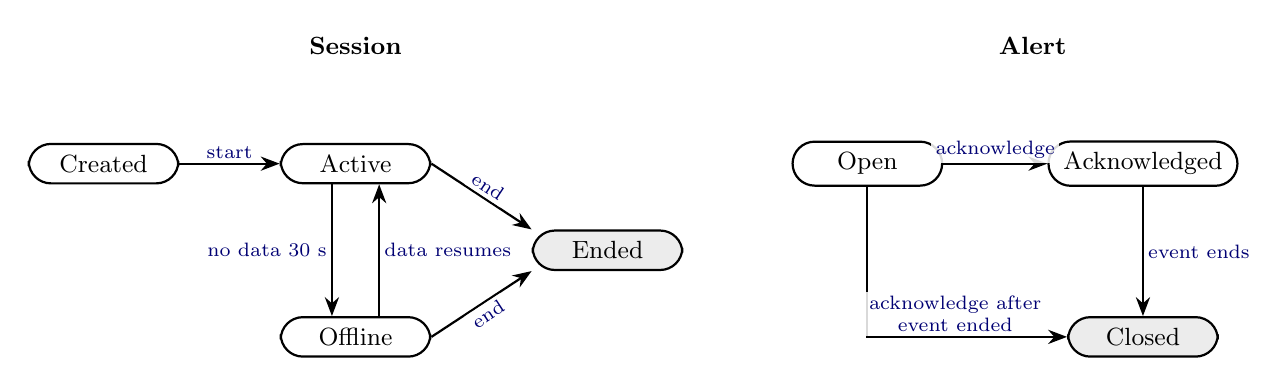
\begin{tikzpicture}[x=1cm,y=1cm, every node/.style={font=\scriptsize}]
  % session machine
  \node[font=\small\bfseries] at (3.4,3.7) {Session};
  \node[box, rounded corners=8pt, minimum width=1.9cm] (s0) at (0.2,2.2) {Created};
  \node[box, rounded corners=8pt, minimum width=1.9cm] (s1) at (3.4,2.2) {Active};
  \node[box, rounded corners=8pt, minimum width=1.9cm] (s2) at (3.4,0) {Offline};
  \node[box, rounded corners=8pt, minimum width=1.9cm, fill=gray!15] (s3) at (6.6,1.1) {Ended};
  \draw[arr] (s0) -- node[lbl,above]{start} (s1);
  \draw[arr] ([xshift=-3mm]s1.south) -- node[lbl,left]{no data 30 s} ([xshift=-3mm]s2.north);
  \draw[arr] ([xshift=3mm]s2.north) -- node[lbl,right]{data resumes} ([xshift=3mm]s1.south);
  \draw[arr] (s1.east) -- node[lbl,above,sloped]{end} (s3.north west);
  \draw[arr] (s2.east) -- node[lbl,below,sloped]{end} (s3.south west);
  % alert machine
  \node[font=\small\bfseries] at (12.0,3.7) {Alert};
  \node[box, rounded corners=8pt, minimum width=1.9cm] (a0) at (9.9,2.2) {Open};
  \node[box, rounded corners=8pt, minimum width=2.4cm] (a1) at (13.4,2.2) {Acknowledged};
  \node[box, rounded corners=8pt, minimum width=1.9cm, fill=gray!15] (a2) at (13.4,0) {Closed};
  \draw[arr] (a0) -- node[lbl,above]{acknowledge} (a1);
  \draw[arr] (a1) -- node[lbl,right]{event ends} (a2);
  \draw[arr] (a0.south) |- node[lbl,above,pos=0.72,align=center]{acknowledge after\\event ended} (a2.west);
\end{tikzpicture}
\caption{State diagrams for a monitoring session and an alert.}
\label{fig:states}
\end{figure}

\section{Feature 6: CV Payload Ingestion}
The ingestion API is the contract between the Python pipeline and the platform. The payload fields are defined in Section~\ref{sec:payload}; the changes required in the pipeline are in Section~\ref{sec:cvi}. Figure~\ref{fig:seq} shows the nominal flow.

\begin{figure}[h!]
\centering
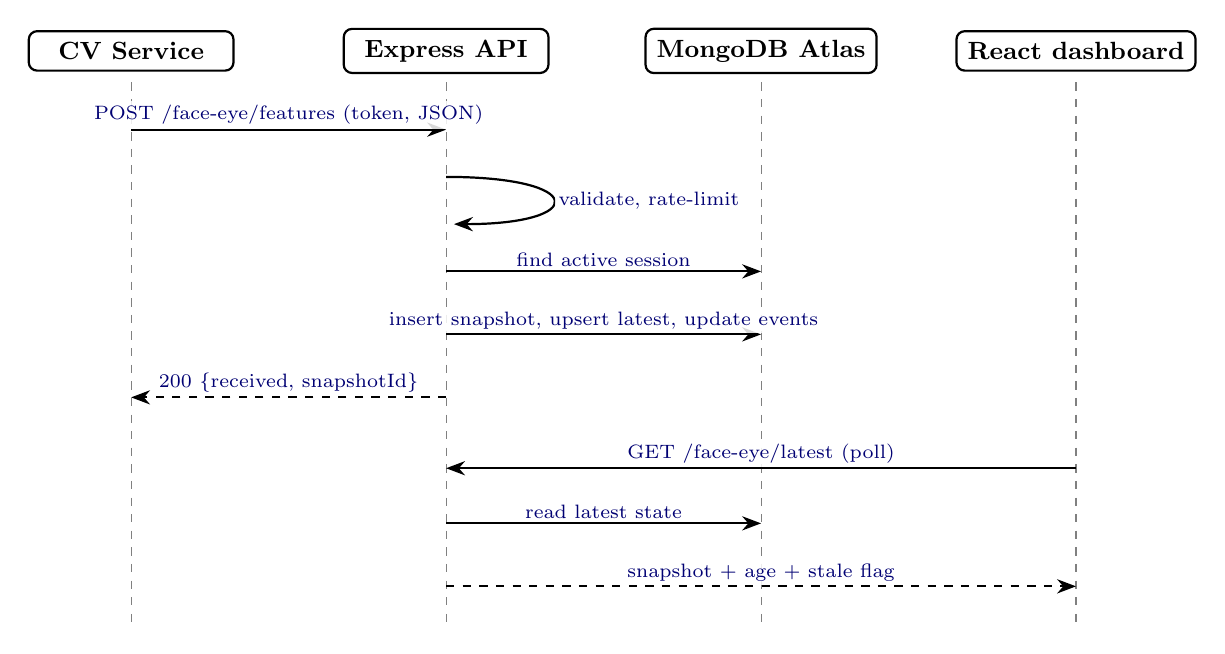
\begin{tikzpicture}[x=1cm,y=1cm, every node/.style={font=\scriptsize}]
  \foreach \x/\n in {1.4/CV Service, 5.4/Express API, 9.4/MongoDB Atlas, 13.4/React dashboard}{
    \node[box, minimum width=2.6cm] at (\x,8.2) {\textbf{\n}};
    \draw[dashed, gray] (\x,7.8) -- (\x,0.9);
  }
  \draw[arr] (1.4,7.2) -- node[lbl,above]{POST /face-eye/features (token, JSON)} (5.4,7.2);
  \draw[arr] (5.4,6.6) .. controls (7.2,6.6) and (7.2,6.0) .. node[lbl,right]{validate, rate-limit} (5.5,6.0);
  \draw[arr] (5.4,5.4) -- node[lbl,above]{find active session} (9.4,5.4);
  \draw[arr] (5.4,4.6) -- node[lbl,above]{insert snapshot, upsert latest, update events} (9.4,4.6);
  \draw[arr, dashed] (5.4,3.8) -- node[lbl,above]{200 \{received, snapshotId\}} (1.4,3.8);
  \draw[arr] (13.4,2.9) -- node[lbl,above]{GET /face-eye/latest (poll)} (5.4,2.9);
  \draw[arr] (5.4,2.2) -- node[lbl,above]{read latest state} (9.4,2.2);
  \draw[arr, dashed] (5.4,1.4) -- node[lbl,above]{snapshot + age + stale flag} (13.4,1.4);
\end{tikzpicture}
\caption{Sequence of a feature payload from the CV Service to the dashboard.}
\label{fig:seq}
\end{figure}

\begin{reqtable}{Ingestion requirements}
\req{FR-ING-01}{\code{POST /api/v1/face-eye/features} shall accept a JSON feature payload from an authenticated CV Service.}{M}
\req{FR-ING-02}{The backend shall validate required fields, types and ranges (Table~\ref{tab:payload}) and reject invalid payloads with 400 or 422 and a list of field errors. An invalid payload shall never be stored as valid.}{M}
\req{FR-ING-03}{The backend shall attach the matching active session, store the capture time (\code{timestamp_unix}) and its own receive time, and use the receive time for ordering.}{M}
\req{FR-ING-04}{The endpoint shall acknowledge a valid payload quickly with \code{\{received, snapshotId, sessionId\}} (target in NFR-PERF-02), because the current sender blocks for up to 1 s per request.}{M}
\req{FR-ING-05}{The latest state shall be updated for every accepted payload, but the history shall be stored at a configurable rate (default one snapshot per second per session) and additionally at every event start and end.}{M}
\req{FR-ING-06}{The latest monitoring state shall be kept separate from historical snapshots (see DR-03).}{M}
\req{FR-ING-07}{\code{GET /api/v1/face-eye/latest} shall return the latest snapshot for a patient together with its age in milliseconds and an \code{isStale} flag computed from the freshness threshold (default 5 s).}{M}
\req{FR-ING-08}{\code{GET /api/v1/face-eye/history} shall return snapshots for a patient or session, filtered by time range and fields, in ascending time order, with a maximum point count (default 2,000) and optional bucket averaging.}{M}
\req{FR-ING-09}{Payloads shall carry \code{schema_version}. A payload without it shall be accepted as the legacy version \code{1.0}; unknown optional fields shall be ignored; an unsupported major version shall be rejected.}{M}
\req{FR-ING-10}{The backend should tolerate duplicate deliveries (same session and sequence number or timestamp) without creating duplicate snapshots.}{S}
\req{FR-ING-11}{\code{POST /api/v1/face-eye/frames} shall accept a multipart upload with the JPEG field \code{frame}; it shall check content type, magic bytes and size (default $\le$ 1 MB) and keep only the latest frame per session in short-lived storage.}{S}
\req{FR-ING-12}{\code{GET /api/v1/face-eye/frames/latest} shall return the latest frame to authorised users only, with \code{Cache-Control: no-store}, or 404 when none exists or it is older than the freshness threshold.}{S}
\req{FR-ING-13}{Frames shall not be written to permanent storage. Any retention feature shall be disabled by default and shall require a documented purpose, access rule and retention period.}{M}
\req{FR-ING-14}{The backend shall store gaze angles in the unit declared by the payload (default radians for version 1.0); conversion to degrees is a display concern.}{M}
\req{FR-ING-15}{The ingestion endpoints shall limit request size (default 16 KB for features) and rate (default 5 requests per second per session) and answer 413 or 429 when exceeded.}{S}
\req{FR-ING-16}{\code{POST /api/v1/face-eye/heartbeat} shall accept a small status message (camera state, face detected, frame rate, baseline ready, pipeline version) and update the session's CV status.}{S}
\req{FR-ING-17}{\code{GET /api/v1/system/health} shall report API status, database connectivity and, for administrators, the age of the last payload per active session.}{M}
\end{reqtable}

\section{Feature 7: Live Face and Eye Monitoring}
This is the core screen. It shows what the pipeline produced, how fresh it is and how reliable it is; it never fills gaps with invented values.
\begin{reqtable}{Live-monitor requirements}
\req{FR-LIVE-01}{The live monitor shall be patient-specific and show the patient, bed, session status and CV Service status.}{M}
\req{FR-LIVE-02}{The monitor shall show the latest preview frame with the pipeline's annotations when available, and a ``No video'' placeholder otherwise.}{S}
\req{FR-LIVE-03}{The monitor shall show the global distress score (0--100) with its severity label: Normal below 20, Mild below 40, Moderate below 60, Severe below 80, Critical otherwise. The thresholds shall be configurable and default to those of the pipeline.}{M}
\req{FR-LIVE-04}{The monitor shall show the pain, fear, fatigue, agitation, tension and respiratory indices (0--100 each). The respiratory index shall be labelled as a visual proxy and not a measured respiration.}{M}
\req{FR-LIVE-05}{The monitor shall show the behaviour state (\code{alert}, \code{drowsy}, \code{eye_closed}, \code{fixation}, \code{scanning}).}{M}
\req{FR-LIVE-06}{The monitor shall show gaze yaw and pitch in degrees, gaze variance, fixation duration in seconds, recent saccade count and eye-contact ratio.}{M}
\req{FR-LIVE-07}{When the behaviour state is \code{eye_closed}, gaze variance and gaze speed shall be shown as ``n/a (eyes closed)'', because the gaze tracker returns zeroed variance and speed fields in that branch.}{M}
\req{FR-LIVE-08}{The monitor shall show face confidence as a feature-quality measure and not as the probability that a clinical interpretation is correct.}{M}
\req{FR-LIVE-09}{The monitor shall show active episode indicators for pain, agitation, fatigue, fear and eye closure and the time of the latest update.}{M}
\req{FR-LIVE-10}{When the payload provides them, the monitor shall also show the 15 AU values, head-pose yaw, pitch and roll, motion energy, asymmetry, PERCLOS and mean and maximum gaze speed. Fields that are absent shall read ``Not provided''.}{S}
\req{FR-LIVE-11}{The monitor shall refresh automatically by polling at a configurable interval (default 2 s). Server-Sent Events or WebSockets may replace polling later.}{M}
\req{FR-LIVE-12}{If the latest snapshot is older than the freshness threshold the monitor shall mark all values as \emph{stale}, grey them out and show the last update time. If nothing has arrived for the offline threshold it shall show ``CV Service offline''. Missing values shall never be shown as zero.}{M}
\req{FR-LIVE-13}{When heartbeats are available, the monitor shall distinguish ``no face detected'' from ``CV Service offline''; otherwise it shall show ``No recent data''.}{S}
\req{FR-LIVE-14}{The monitor shall show whether the baseline is ready; while it is not, values shall carry a ``calibrating'' note.}{S}
\req{FR-LIVE-15}{Users shall be able to switch between their rostered patients from the monitor.}{M}
\req{FR-LIVE-16}{The interface shall not display posture, audio, vitals (heart rate, SpO$_2$, blood pressure), seizure score, AI risk-prediction or lab panels. A placeholder, where used, shall read ``Not available in this version''.}{M}
\req{FR-LIVE-17}{Every monitoring screen shall show the notice ``Research prototype --- visual estimates are not a diagnosis''.}{M}
\end{reqtable}

\section{Feature 8: Monitoring Events and Alert Centre}
The pipeline's episode detector reports five episode types as flags. The platform turns each flag transition into a stored \emph{event}, and selected events into \emph{alerts} that staff acknowledge.
\begin{reqtable}{Event and alert requirements}
\req{FR-EVT-01}{When an episode flag (pain, agitation, fatigue, fear, eye closure) changes from false to true, the backend shall create an event with its start time; when it changes to false the backend shall close the event and record the end time and duration.}{M}
\req{FR-EVT-02}{Each event shall store type, patient, session, start, end, duration, the peak value of the related index and its status (active or completed).}{M}
\req{FR-EVT-03}{\code{GET /api/v1/face-eye/events} shall list events filtered by patient, session, type, status and time range.}{M}
\req{FR-EVT-04}{The backend shall raise an alert when an event of a configured type starts and when the global distress stays at or above the Severe threshold for a configured time (default 10 s). Rules are set in server configuration; editing rules in the interface is future scope.}{M}
\req{FR-EVT-05}{The alert centre shall list alerts newest first with severity, patient, bed, description, time and status, and shall keep unacknowledged alerts visible until they are acknowledged.}{M}
\req{FR-EVT-06}{A doctor or nurse responsible for the patient shall be able to acknowledge an alert; the system shall record the user and time.}{M}
\req{FR-EVT-07}{The backend should suppress repeated alerts of the same type for the same patient within a cool-down window (default 60 s).}{S}
\req{FR-EVT-08}{Alert text shall describe the configured visual rule that fired (for example ``Pain-related facial behaviour episode started'') and shall not state a diagnosis.}{M}
\req{FR-EVT-09}{The interface may show a toast and an optional sound for new Severe or Critical alerts.}{C}
\req{FR-EVT-10}{The ``Emergency call'' button shall record a call request and notify on-duty staff in the platform. It shall not contact external emergency services.}{C}
\end{reqtable}

\section{Feature 9: Historical Analytics}
Historical views let staff review how recorded observations changed over a session. They show recorded values and events only.
\begin{reqtable}{Historical-analytics requirements}
\req{FR-HIST-01}{Authorised users shall be able to select a patient, session and time range and see a time-series chart of the global distress score and of any single index.}{M}
\req{FR-HIST-02}{The history view shall list the events of the selected range with type, start, end and duration, aligned with the chart.}{M}
\req{FR-HIST-03}{Observations shall be ordered by timestamp. Gaps in data shall appear as gaps in the chart and shall not be interpolated or filled with zero.}{M}
\req{FR-HIST-04}{The history view shall offer eye metrics (gaze variance, fixation duration, eye-contact ratio and, when provided, PERCLOS) and the share of time spent in each behaviour state.}{S}
\req{FR-HIST-05}{For each session the system shall show a summary: mean and maximum global distress, number of events by type, and data coverage (share of the session with fresh data).}{S}
\req{FR-HIST-06}{Long ranges shall be returned as bucket averages so that one response never exceeds the point limit of FR-ING-08.}{S}
\req{FR-HIST-07}{Authorised roles shall be able to export a session's snapshots and events as CSV; exports shall not contain video frames.}{S}
\req{FR-HIST-08}{Administrators shall see aggregate analytics (patient counts, sessions, events per day, occupancy) without patient identities.}{S}
\req{FR-HIST-09}{Charts shall be based on recorded observations only; the interface shall not present trends as diagnoses or predictions.}{M}
\end{reqtable}

\section{Feature 10: Doctor Workspace}
The doctor workspace combines the roster, the currently monitored patient and the alert centre, as in the doctor dashboard of the reference video.
\begin{reqtable}{Doctor-workspace requirements}
\req{FR-DOC-01}{The doctor dashboard shall show the doctor's active roster (name, ward or bed, selection state) and a ``currently monitoring'' panel with the selected patient's latest distress score and status.}{M}
\req{FR-DOC-02}{The dashboard shall include the alert centre for the doctor's patients.}{M}
\req{FR-DOC-03}{The dashboard shall link to the live monitor and the history of each rostered patient.}{M}
\req{FR-DOC-04}{A doctor shall be able to add and edit timestamped clinical notes for an assigned patient; each note shall record its author.}{S}
\req{FR-DOC-05}{A doctor shall be able to create task and medication-schedule entries for assigned patients (record keeping only, see BR-04).}{S}
\req{FR-DOC-06}{A doctor shall be able to publish a short status note that the linked family account can read.}{C}
\req{FR-DOC-07}{A doctor shall be able to request a shift handoff, which creates a summary of open alerts, pending tasks and recent notes for the incoming doctor.}{C}
\end{reqtable}

\section{Feature 11: Nurse Workspace}
The nurse workspace supports shift check-in, an overview of assigned beds and tasks, and the medication schedule.
\begin{reqtable}{Nurse-workspace requirements}
\req{FR-NUR-01}{A nurse shall check in to a shift (selected from the shifts defined by the administrator) before using the nurse station, and shall be able to check out; check-in and check-out times shall be stored.}{S}
\req{FR-NUR-02}{The nurse overview shall show assigned beds, pending medication, tasks due, time since the last recorded check, the nurse's patients and open alerts.}{S}
\req{FR-NUR-03}{A nurse shall be able to open the live monitor of each assigned patient and acknowledge alerts.}{M}
\req{FR-NUR-04}{A nurse shall be able to create, edit, complete and delete care tasks for assigned patients, each with a due time and status (for example ``Wound care dressing change'').}{S}
\req{FR-NUR-05}{A nurse shall be able to add scheduled medication entries (name, dose, route, patient, due time) and mark an entry as \emph{Given}; the system shall record the user and time.}{S}
\req{FR-NUR-06}{Medication entries are records only: the system shall not recommend doses, check interactions or send orders (BR-04).}{M}
\req{FR-NUR-07}{Nurse login, check-in, check-out and completed tasks shall be visible to administrators as staff activity.}{S}
\end{reqtable}

\section{Feature 12: Administrator Workspace}
The administrator workspace covers users, rooms, staffing and system status. It does not show live clinical video.
\begin{reqtable}{Administrator-workspace requirements}
\req{FR-ADM-01}{An administrator shall be able to create, edit and disable user accounts, assign roles, link family accounts to a patient and reset credentials.}{M}
\req{FR-ADM-02}{An administrator shall be able to define floors, rooms and beds and see each bed as available, occupied or critical.}{S}
\req{FR-ADM-03}{An administrator shall be able to allocate a patient to a free bed under a selected doctor, and to deallocate; the ``critical'' flag shall be a manual marker set by authorised staff and shall not be computed from the CV scores.}{S}
\req{FR-ADM-04}{The staffing view shall list nurses and doctors on duty with their shifts, and show a nurse's recent activity (login, check-in, tasks, check-out).}{S}
\req{FR-ADM-05}{The department view may group departments, doctors, nurses and their patients.}{C}
\req{FR-ADM-06}{The system-status view shall show API health, database status and, for each active session, the CV Service status and the age of its last payload.}{M}
\req{FR-ADM-07}{The admin dashboard shall show the alert centre in a read-only form that links to the responsible clinicians.}{S}
\req{FR-ADM-08}{Equipment inventory shown in the reference video is out of scope for Version 1.0.}{--}
\end{reqtable}

\section{Feature 13: Family Workspace}
The family workspace is a deliberately small, read-only view of information that a doctor has chosen to release.
\begin{reqtable}{Family-workspace requirements}
\req{FR-FAM-01}{A family account shall be linked by an administrator to one patient and shall see only that patient.}{C}
\req{FR-FAM-02}{The ``My Recovery'' view shall be read-only and show the patient's name, ward and the status notes released by a doctor.}{C}
\req{FR-FAM-03}{The family view shall not show raw indices, video frames, alerts, events or other patients' data.}{C}
\req{FR-FAM-04}{A family account shall be activated only after an administrator records that the patient or guardian has consented to family access.}{C}
\end{reqtable}

\section{Feature 14: Messaging, Emergency Call and Handoff}
These features follow the messages tab and header buttons of the reference video. They are low priority.
\begin{reqtable}{Messaging requirements}
\req{FR-MSG-01}{Staff shall be able to send text messages to other staff accounts and read their threads; a family user shall be able to message the care team only.}{C}
\req{FR-MSG-02}{The system may post system messages for shift check-in and check-out, as shown in the reference video.}{C}
\req{FR-MSG-03}{Messages shall not be used to transmit CV frames or raw payloads.}{C}
\end{reqtable}

\section{Feature 15: Audit Logging}
Audit logging records who did what, so that access to patient information can be reviewed.
\begin{reqtable}{Audit requirements}
\req{FR-AUD-01}{The system shall write an append-only audit entry (user, role, action, object, time, outcome) for sign-in and sign-out, role changes, patient-record access and edits, session start and end, alert acknowledgement and data export.}{S}
\req{FR-AUD-02}{Administrators shall be able to view and filter the audit log; no role shall be able to edit or delete entries through the interface.}{S}
\req{FR-AUD-03}{Audit entries shall not contain passwords, tokens, video frames or free-text clinical content.}{S}
\end{reqtable}

\section{CV Service Integration Requirements}\label{sec:cvi}
The audit of the repository shows that the current pipeline cannot talk to the new API without changes. This section lists those changes. They are requirements on the \emph{existing Python component} and are tracked as part of this project.
\begin{reqtable}{Required changes in the Face + Eye Pipeline}
\req{CVI-01}{Replace the hard-coded constants \code{ENABLE_BACKEND}, \code{BACKEND_URL} and \code{STREAM_URL} in \code{backend_sender.py} by configuration (environment variables) that point to \code{/api/v1/face-eye/features} and \code{/api/v1/face-eye/frames}. The checked-in values (\code{172.20.10.2:8000}, \code{/api/face-eye/features}, \code{/api/stream/face}) match neither the in-repo FastAPI service nor this contract.}{M}
\req{CVI-02}{Extend the payload as defined in Table~\ref{tab:payload}: add \code{schema_version} and \code{units}; add the optional AUs, head pose, motion, EAR, PERCLOS, gaze-speed, baseline and frame-rate fields that the pipeline already computes.}{M}
\req{CVI-03}{Send payloads from a worker thread through a bounded queue, so that a slow or unreachable backend can no longer stall the camera loop. The drop policy (oldest first) and drop counters shall be documented.}{M}
\req{CVI-04}{Check the HTTP status of every request (for example with \code{raise_for_status}), log failures with counters, and describe delivery as best-effort. The current code has no retry, no durable queue and no delivery confirmation.}{M}
\req{CVI-05}{Send the service token in the \code{Authorization} header of every request.}{M}
\req{CVI-06}{Send a heartbeat every 5 s (camera state, face detected, frame rate, baseline ready, pipeline version) even when no face is tracked.}{S}
\req{CVI-07}{Limit feature posts to a configurable rate (default 2 per second, maximum 5) independent of the camera frame rate.}{S}
\req{CVI-08}{Limit preview frames to a configurable size and rate (default width $\le$ 640 px, JPEG quality about 70, $\le$ 2 frames per second) and add the \code{patient_id} form field to the multipart request.}{S}
\req{CVI-09}{Compute gaze durations from timestamps or the measured frame rate instead of the fixed 30 FPS assumption, and reconcile the saccade-window comment (150 frames) with its stated meaning.}{S}
\req{CVI-10}{Use the configurable camera index of \code{CameraConfig} instead of the fixed device 0.}{S}
\req{CVI-11}{Align the JSONL log with the CSV and payload by adding gaze fields and the behaviour state.}{C}
\end{reqtable}

\section{External Interface Requirements}
\begin{idtable}{Interface requirements}
\idr{IR-UI-01}{The frontend shall be a responsive React SPA that works from 360 px to 1920 px wide and follows the layout and navigation of the reference video (Section~\ref{sec:ui}).}
\idr{IR-UI-02}{Colour shall not be the only carrier of meaning: status chips and severity shall also show text.}
\idr{IR-HW-01}{The CV Service shall read frames from a USB or built-in RGB camera (OpenCV \code{VideoCapture}) on the host machine.}
\idr{IR-HW-02}{The CV host shall be able to run MediaPipe Face Mesh and L2CS-Net inference; a CUDA GPU is optional.}
\idr{IR-SW-01}{The CV Service shall call the backend over HTTPS using JSON, plus multipart/form-data for preview frames.}
\idr{IR-SW-02}{The frontend shall call the backend over HTTPS using JSON. The backend shall allow cross-origin requests only from the configured frontend origin.}
\idr{IR-SW-03}{The backend shall access MongoDB Atlas through the official driver or Mongoose with a least-privilege database user.}
\idr{IR-COM-01}{All traffic shall use TLS. Timestamps in API responses shall be ISO~8601 in UTC; the CV payload carries \code{timestamp_unix} in seconds.}
\end{idtable}

\section{REST API Summary}\label{sec:api}
All endpoints are under \code{/api/v1}. The list below extends the proposal's API with the endpoints needed by the features above; none of it exists yet and it is implemented during development.

\begin{itemize}
  \item \textbf{Format:} JSON, UTF-8. Lists use \code{limit} and \code{cursor} parameters.
  \item \textbf{Errors:} \code{\{ "error": \{ "code", "message", "details", "requestId" \} \}} with status 400, 401, 403, 404, 409, 413, 422, 429 or 503 as appropriate.
  \item \textbf{Authentication:} user token (cookie or bearer) for people; service token in \code{Authorization: Bearer} for the CV Service.
  \item \textbf{Roles:} P = public, A = Admin, D = Doctor, N = Nurse, F = Family, S = CV Service.
\end{itemize}

\begin{longtable}{@{}>{\ttfamily\footnotesize}p{1.7cm}>{\ttfamily\footnotesize}p{5.4cm}>{\raggedright\arraybackslash}p{4.9cm}>{\raggedright\arraybackslash}p{2.2cm}@{}}
\caption{REST API summary}\label{tab:api}\\
\toprule \textbf{Method} & \textbf{Path} & \textbf{Purpose} & \textbf{Roles}\\ \midrule \endfirsthead
\toprule \textbf{Method} & \textbf{Path} & \textbf{Purpose} & \textbf{Roles}\\ \midrule \endhead
\bottomrule \endfoot
POST & /auth/register & Create a user (admin only) & A\\
POST & /auth/login & Sign in & P\\
POST & /auth/logout & Sign out & all\\
GET & /auth/me & Current user and role & all\\
GET, PATCH & /users, /users/:userId & List users; edit, disable, reset & A\\
GET, POST & /patients & List, create patients & A, D, N(R)\\
GET, PATCH, DELETE & /patients/:patientId & Read, update, archive & A, D, N(R)\\
GET, POST & /patients/:patientId/sessions & List, start sessions & D, N\\
GET, PATCH & /sessions/:sessionId & Read, end a session & D, N\\
POST & /face-eye/features & Submit feature payload & S\\
POST & /face-eye/heartbeat & Submit CV status & S\\
POST & /face-eye/frames & Submit preview frame (multipart) & S\\
GET & /face-eye/latest & Latest snapshot with age and stale flag & D, N\\
GET & /face-eye/frames/latest & Latest preview frame & D, N\\
GET & /face-eye/history & Snapshots by time range & D, N\\
GET & /face-eye/events & Monitoring events & D, N, A(R)\\
GET & /alerts & Alert list & A(R), D, N\\
POST & /alerts/:alertId/acknowledge & Acknowledge an alert & D, N\\
GET, POST & /patients/:patientId/tasks & List, create care tasks & A(R), D, N\\
PATCH, DELETE & /tasks/:taskId & Update, complete, delete a task & D, N\\
GET, POST & /patients/:patientId/medications & List, add medication entries & D, N\\
PATCH & /medications/:medId & Mark as given, edit & D, N\\
GET, POST & /patients/:patientId/notes & List, add clinical notes & D, N(R)\\
GET, PATCH & /beds & List beds; allocate, deallocate, set critical & A, D(R), N(R)\\
POST & /shifts/check-in, /shifts/check-out & Record shift start or end & D, N\\
GET, POST & /messages & Read, send messages & A, D, N, F\\
GET & /dashboard/summary & Counts, active sessions, recent events & A, D, N\\
GET & /system/health & Health check (details for admin) & P, A\\
GET & /audit-logs & Audit log & A\\
\end{longtable}

\section{CV Payload Contract}\label{sec:payload}
Table~\ref{tab:payload} defines payload version~1. The first group is what the checked-in pipeline already sends (version \code{1.0}, no \code{schema_version} field). The second group requires the changes of CVI-02. Value ranges marked ``to be confirmed'' shall be fixed in the integration audit (Phase 5). An example is given in Appendix~\ref{app:json}.

\begin{longtable}{@{}>{\ttfamily\footnotesize}p{3.6cm}>{\raggedright\arraybackslash}p{1.7cm}>{\raggedright\arraybackslash}p{3.7cm}c>{\raggedright\arraybackslash}p{3.3cm}@{}}
\caption{CV feature payload, version 1}\label{tab:payload}\\
\toprule \textbf{Field} & \textbf{Type} & \textbf{Unit / range} & \textbf{Req.} & \textbf{Current pipeline}\\ \midrule \endfirsthead
\toprule \textbf{Field} & \textbf{Type} & \textbf{Unit / range} & \textbf{Req.} & \textbf{Current pipeline}\\ \midrule \endhead
\bottomrule \endfoot
\multicolumn{5}{@{}l}{\textit{Group 1 --- fields in the checked-in payload}}\\ \midrule
patient_id & string & patient reference, e.g.\ P001 & Yes & sent\\
timestamp_unix & number & seconds since epoch, UTC & Yes & sent\\
global_distress & number & 0--100 & Yes & sent\\
pain_index, fear_index, fatigue_index, agitation_index, tension_index, respiratory_index & number & 0--100 each & Yes & sent\\
behavior_state & string & alert, drowsy, eye_closed, fixation, scanning & Yes & sent\\
gaze_yaw, gaze_pitch & number or null & radians & Yes & sent\\
gaze_variance & number & unit to be confirmed & Yes & sent\\
fixation_duration & number & seconds (30 FPS assumed in code) & Yes & sent\\
recent_saccades & integer & count, $\ge$ 0 & Yes & sent\\
eye_contact_ratio & number & ratio & Yes & sent\\
episode_pain, episode_agitation, episode_fatigue, episode_fear, episode_eye_closure & boolean & --- & Yes & sent\\
face_confidence & number & range to be confirmed & Yes & sent\\ \midrule
\multicolumn{5}{@{}l}{\textit{Group 2 --- additions (CVI-02)}}\\ \midrule
schema_version & string & e.g.\ "1.1" & Yes & new\\
units & object & declares gaze unit and similar & Should & new\\
baseline_ready & boolean & --- & Should & in CSV/JSONL, not sent\\
fps, pipeline_version & number, string & measured frame rate; tag or commit & Should & new\\
seq & integer & increasing per session & Optional & new\\
au & object & AU4 to AU43 (15 values) and mar & Optional & computed, not sent\\
head_pose & object & yaw, pitch, roll in degrees & Optional & computed, not sent\\
motion_energy, facial_asymmetry & number & 0--1; normalised & Optional & computed, not sent\\
ear_avg, eye_closed & number, boolean & eye aspect ratio; closure flag & Optional & computed, not sent\\
perclos & number & 0--1 & Optional & computed, not sent\\
mean_gaze_speed, max_gaze_speed & number & unit to be confirmed & Optional & in CSV, not sent\\
\end{longtable}

\section{Data Requirements}\label{sec:data}
MongoDB Atlas stores the data in the collections of Figure~\ref{fig:data} and Table~\ref{tab:collections}. The final schema may change with implementation; the requirements below remain.

\begin{figure}[h!]
\centering
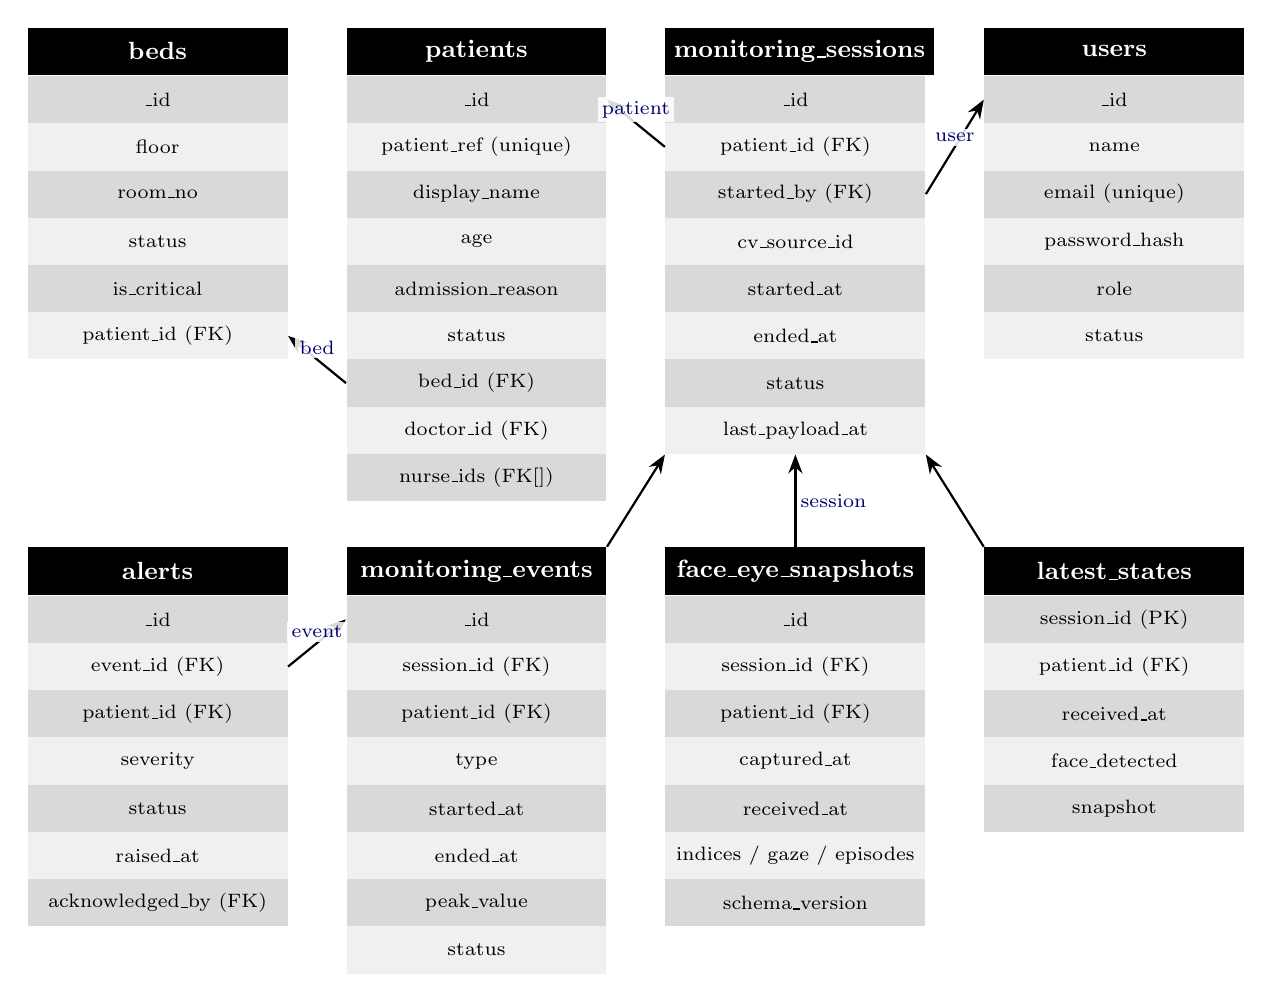
\begin{tikzpicture}[x=1cm,y=1cm]
  \begin{scope}[gra/.append style={font=\scriptsize}, grb/.append style={font=\scriptsize}]
  \stack{be}{0,0}{3.3cm}{beds}{_id,floor,room_no,status,is_critical,patient_id (FK)}
  \stack{pa}{4.05,0}{3.3cm}{patients}{_id,patient_ref (unique),display_name,age,admission_reason,status,bed_id (FK),doctor_id (FK),nurse_ids (FK[])}
  \stack{se}{8.1,0}{3.3cm}{monitoring_sessions}{_id,patient_id (FK),started_by (FK),cv_source_id,started_at,ended_at,status,last_payload_at}
  \stack{us}{12.15,0}{3.3cm}{users}{_id,name,email (unique),password_hash,role,status}
  \stack{al}{0,-6.6}{3.3cm}{alerts}{_id,event_id (FK),patient_id (FK),severity,status,raised_at,acknowledged_by (FK)}
  \stack{ev}{4.05,-6.6}{3.3cm}{monitoring_events}{_id,session_id (FK),patient_id (FK),type,started_at,ended_at,peak_value,status}
  \stack{sn}{8.1,-6.6}{3.3cm}{face_eye_snapshots}{_id,session_id (FK),patient_id (FK),captured_at,received_at,indices / gaze / episodes,schema_version}
  \stack{ls}{12.15,-6.6}{3.3cm}{latest_states}{session_id (PK),patient_id (FK),received_at,face_detected,snapshot}
  \end{scope}
  \draw[arr] (pa-7.west) -- node[lbl,above,pos=0.5]{bed} (be-6.east);
  \draw[arr] (se-2.west) -- node[lbl,above,pos=0.5]{patient} (pa-1.east);
  \draw[arr] (se-3.east) -- node[lbl,above,pos=0.5]{user} (us-1.west);
  \draw[arr] (sn-h.north) -- node[lbl,right]{session} (se-8.south);
  \draw[arr] (ev-h.north east) -- (se-8.south west);
  \draw[arr] (ls-h.north west) -- (se-8.south east);
  \draw[arr] (al-2.east) -- node[lbl,above,pos=0.5]{event} (ev-1.west);
\end{tikzpicture}
\caption{Core data model (collections and foreign-key references). Administrative collections are listed in Table~\ref{tab:collections}.}
\label{fig:data}
\end{figure}

\begin{longtable}{@{}>{\ttfamily\footnotesize}p{3.4cm}>{\raggedright\arraybackslash}p{5.4cm}>{\raggedright\arraybackslash}p{5.8cm}@{}}
\caption{Collections, purpose and indexes}\label{tab:collections}\\
\toprule \textbf{Collection} & \textbf{Purpose} & \textbf{Indexes and retention}\\ \midrule \endfirsthead
\toprule \textbf{Collection} & \textbf{Purpose} & \textbf{Indexes and retention}\\ \midrule \endhead
\bottomrule \endfoot
users & Accounts, roles, status & unique email; role\\ \midrule
patients & Minimal patient records & unique patient_ref; status; doctor_id; nurse_ids\\ \midrule
beds & Floors, rooms, allocation & unique (floor, room_no); status\\ \midrule
monitoring_sessions & One document per session & (patient_id, started_at desc); at most one active per patient\\ \midrule
latest_states & Latest state per session & unique session_id\\ \midrule
face_eye_snapshots & Time-ordered feature history & (session_id, received_at), (patient_id, received_at); TTL on received_at (default 30 days); time-series collection allowed\\ \midrule
monitoring_events & Events from episode flags & (session_id, started_at), (patient_id, started_at), status\\ \midrule
alerts & Alerts and acknowledgements & (status, raised_at desc), (patient_id, raised_at)\\ \midrule
care_tasks, medication_schedules, clinical_notes & Administrative and clinical records & (patient_id, due_at); (patient_id, created_at)\\ \midrule
shift_records, messages & Staff activity, messaging & (user_id, check_in_at); (thread, created_at)\\ \midrule
audit_logs & Append-only audit trail & (user_id, at), (object, at); retention set by policy\\
\end{longtable}

\begin{idtable}{Data requirements}
\idr{DR-01}{Every document shall have a unique identifier and creation and update timestamps; times shall be stored in UTC.}
\idr{DR-02}{Frequently queried fields (patient references, session identifiers, timestamps, status) shall be indexed as in Table~\ref{tab:collections}.}
\idr{DR-03}{The latest monitoring state shall be stored in \code{latest_states}, separate from historical snapshots, so that the live view never scans history.}
\idr{DR-04}{Each snapshot shall store the payload schema version and the fields received; fields not provided shall be stored as absent, not as zero.}
\idr{DR-05}{Snapshots shall expire through a TTL index (default 30 days, configurable). Events, alerts and clinical records follow a retention policy to be agreed with the supervisor and ethics adviser.}
\idr{DR-06}{Referential integrity shall be enforced in the application layer. Patients and users shall be archived or disabled rather than deleted, so that history keeps its references.}
\idr{DR-07}{Passwords shall be stored as hashes only. Video frames shall not be stored in the database.}
\idr{DR-08}{Only the fields listed in the schema shall be stored; the minimum-data rule of FR-PAT-06 applies to every collection.}
\end{idtable}

\chapter{Other Nonfunctional Requirements}
Numeric values in this chapter are initial design targets (Section~\ref{sec:conventions}). They shall be measured during testing and reported as measured values.

\section{Performance Requirements}
These requirements keep the live view responsive and make sure that sending data to the platform does not slow the camera pipeline.
\begin{reqtable}{Performance requirements}
\req{NFR-PERF-01}{Under nominal load, a payload accepted by the backend shall appear on an open live monitor within 3 s at the 95th percentile (polling interval of 2 s included).}{M}
\req{NFR-PERF-02}{The feature-ingestion endpoint shall return its acknowledgement within 200 ms at the 95th percentile, excluding network time, so that the synchronous sender is not delayed.}{M}
\req{NFR-PERF-03}{Read endpoints for the latest state, alerts and dashboard summary shall respond within 500 ms at the 95th percentile; a history query for 24 hours of bucket-averaged data shall respond within 2 s.}{S}
\req{NFR-PERF-04}{The prototype shall support at least 5 concurrent active sessions and 25 concurrent dashboard users, each session posting at most 5 payloads per second.}{S}
\req{NFR-PERF-05}{The frontend shall load its first screen within 3 s on a broadband connection, use code splitting per workspace, and keep polling timers paused while the browser tab is hidden.}{S}
\req{NFR-PERF-06}{Enabling the backend connection shall not reduce the pipeline's processing rate measurably; the integration test shall compare frame rates with and without sending.}{M}
\end{reqtable}

\section{Security Requirements}
Only registered users can enter the system, and each user can perform only the actions of their role.
\begin{reqtable}{Security requirements}
\req{NFR-SEC-01}{All traffic between browser, CV Service, backend and database shall use TLS; the backend shall send security headers (HSTS and the standard \code{helmet} set).}{M}
\req{NFR-SEC-02}{Passwords shall use bcrypt with cost at least 12, or Argon2id.}{M}
\req{NFR-SEC-03}{Tokens shall be signed with a secret from the environment and be short-lived. Cookies shall be HttpOnly, Secure and SameSite, with protection against cross-site request forgery.}{M}
\req{NFR-SEC-04}{Authorisation shall be enforced on the server by role and by object (assignment), following the principle of least privilege.}{M}
\req{NFR-SEC-05}{All input shall be validated against a schema; query operators in user input shall be rejected to prevent NoSQL injection; output shall be encoded to prevent cross-site scripting; cross-origin access shall be restricted to the frontend origin.}{M}
\req{NFR-SEC-06}{Secrets (database URI, token secrets) shall be stored in environment variables and never committed to the repository; a \code{.env.example} shall document them.}{M}
\req{NFR-SEC-07}{The CV Service shall use its own service token, accepted only by the ingestion endpoints, revocable without affecting users.}{M}
\req{NFR-SEC-08}{Sign-in and ingestion endpoints shall be rate-limited.}{S}
\req{NFR-SEC-09}{The database user shall have only the permissions the backend needs, and the Atlas network access list shall be restricted to what the deployment requires.}{S}
\req{NFR-SEC-10}{Logs shall not contain passwords, tokens, video frames or free-text clinical content.}{M}
\req{NFR-SEC-11}{Dependencies shall be checked for known vulnerabilities (for example \code{npm audit}) before each release.}{S}
\end{reqtable}

\section{Privacy and Data Protection}
The system observes patients by camera and stores clinical records, so privacy is a design requirement from the start.
\begin{reqtable}{Privacy requirements}
\req{NFR-PRV-01}{The system shall collect and store only the minimum patient information needed for the project (FR-PAT-06, DR-08).}{M}
\req{NFR-PRV-02}{Camera frames shall not be stored permanently by default (FR-ING-13).}{M}
\req{NFR-PRV-03}{Retention periods shall be configurable and documented (DR-05).}{M}
\req{NFR-PRV-04}{Access to patient data shall be limited by role and assignment and recorded in the audit log (FR-AUD-01).}{S}
\req{NFR-PRV-05}{Development and testing shall use volunteers, recorded or synthetic data. Real patient data shall be used only after ethics approval and consent (A-07).}{M}
\req{NFR-PRV-06}{Where possible the interface shall show the patient reference instead of the full name on shared screens.}{C}
\req{NFR-PRV-07}{The project shall not claim compliance with HIPAA, GDPR or similar regulations. The design supports future compliance work but does not establish it.}{M}
\end{reqtable}

\section{Reliability and Availability}
A monitoring tool must make its own failures visible. These requirements cover failure handling and the honest display of missing data.
\begin{reqtable}{Reliability requirements}
\req{NFR-REL-01}{The platform shall degrade gracefully: if the CV Service is offline the dashboards shall show that state and the record-keeping features shall keep working.}{M}
\req{NFR-REL-02}{If the database is unavailable the API shall answer 503 with a clear error code and recover without restart when the database returns.}{M}
\req{NFR-REL-03}{Missing, stale and unavailable data shall be shown as such and never replaced by zero (FR-LIVE-12, DR-04).}{M}
\req{NFR-REL-04}{The backend shall handle missing faces, invalid frames, malformed payloads and disconnected services without crashing, and shall log them with a request identifier.}{M}
\req{NFR-REL-05}{The backend shall apply request timeouts (default 10 s) and the frontend shall show loading, empty and error states for every data view.}{S}
\req{NFR-REL-06}{The system shall offer a health endpoint for monitoring and automatic restart (FR-ING-17).}{M}
\req{NFR-REL-07}{Automated database backups shall be enabled where the Atlas plan supports them.}{C}
\end{reqtable}

\section{Usability and Accessibility}
Doctors and nurses use the interface under time pressure, often on tablets.
\begin{reqtable}{Usability requirements}
\req{NFR-USE-01}{The interface shall be responsive from 360 px to 1920 px and usable by touch on tablets; touch targets shall be at least 44 px.}{M}
\req{NFR-USE-02}{The layout and wording shall be consistent across workspaces: one navigation pattern, one set of status chips, units shown next to every value.}{S}
\req{NFR-USE-03}{The interface shall target WCAG 2.1 level AA for colour contrast and keyboard operation of the main flows.}{S}
\req{NFR-USE-04}{Times shall be shown in the user's local time zone with the UTC value available on hover.}{S}
\req{NFR-USE-05}{A first-time doctor or nurse shall be able to open the live monitor of an assigned patient within three actions after sign-in.}{S}
\req{NFR-USE-06}{The interface language is English.}{M}
\end{reqtable}

\section{Maintainability and Portability}
The code base is developed by a small team and extended after the project, so it must be easy to understand and reproduce.
\begin{reqtable}{Maintainability requirements}
\req{NFR-MNT-01}{The backend shall be organised in routes, controllers, services and models, with centralised error handling and request validation.}{M}
\req{NFR-MNT-02}{The repository shall use a linter and formatter, a README with set-up steps, and a \code{.env.example} for each component.}{M}
\req{NFR-MNT-03}{The API shall be documented in an OpenAPI description that matches Table~\ref{tab:api} and Table~\ref{tab:payload}.}{S}
\req{NFR-MNT-04}{Thresholds, intervals and retention periods named in this SRS shall be configuration values, not constants in code.}{M}
\req{NFR-MNT-05}{The frontend and backend shall run unchanged on any machine with the documented Node.js version and the environment variables set.}{S}
\end{reqtable}

\section{Software Quality Attributes}
Quality is maintained by testing during development, not only at the end. Database, logical, API and user-interface tests are required, and each requirement in this document is written to be verifiable.
\begin{reqtable}{Testing requirements}
\req{NFR-TST-01}{Unit tests shall cover validation, authorisation rules, event derivation, freshness and stale logic, and the data-access layer.}{M}
\req{NFR-TST-02}{API tests shall cover every endpoint of Table~\ref{tab:api} for success, validation errors, 401, 403, 404 and 409 cases.}{M}
\req{NFR-TST-03}{A contract test shall check that the payload of Table~\ref{tab:payload} accepted by the backend is the same one the frontend renders, so that a field-name mismatch cannot go unnoticed.}{M}
\req{NFR-TST-04}{A CV simulator shall replay recorded or synthetic payloads (including no-face gaps, an eye-closed period and a stopped service) against the API so that the full flow can be tested without a camera.}{M}
\req{NFR-TST-05}{Integration tests shall cover the whole path camera or simulator $\rightarrow$ API $\rightarrow$ MongoDB $\rightarrow$ dashboard, including camera disconnect, no face, CV Service stopped and database unavailable.}{M}
\req{NFR-TST-06}{UI tests shall cover sign-in per role, workspace guards, live monitor states (live, stale, offline, no data) and alert acknowledgement.}{S}
\req{NFR-TST-07}{A load test shall check the targets of NFR-PERF-01 to NFR-PERF-04 and the results shall be recorded.}{S}
\req{NFR-TST-08}{Any statement about CV accuracy requires annotated evaluation data and a separate experimental method. Successful integration alone shall not be presented as clinical validity.}{M}
\end{reqtable}

\section{Business Rules}
The platform stores monitoring information and supports staff; it does not make clinical decisions. These rules govern every screen, report and demonstration.
\begin{idtable}{Business rules}
\idr{BR-01}{The system is a research and monitoring-support prototype. It is not a validated medical device and does not diagnose, prescribe or replace physiological measurement or professional judgement.}
\idr{BR-02}{Every index, behaviour state, severity label and episode shall be presented as a visual heuristic derived from facial and eye features, with the software-defined thresholds of the pipeline.}
\idr{BR-03}{No value shall be fabricated. A module without a data source is hidden or marked ``Not available in this version''. Illustrative content is labelled as sample data.}
\idr{BR-04}{Tasks and medication entries are administrative records. The system shall not recommend, schedule automatically or alter treatment.}
\idr{BR-05}{Only authorised staff responsible for a patient may acknowledge that patient's alerts.}
\idr{BR-06}{Camera frames are live previews and are not stored unless a documented retention feature is enabled.}
\idr{BR-07}{Changes to severity thresholds, alert rules and retention periods are configuration changes and shall be recorded in the project documentation.}
\idr{BR-08}{Patient and user records are archived or disabled, never deleted through the interface.}
\idr{BR-09}{Accuracy or performance claims about the CV indices shall be made only with annotated evaluation data (NFR-TST-08).}
\end{idtable}

\chapter{Other Requirements}
The ICU Monitoring Platform will need maintenance, because the requirements will change as the CV pipeline is audited and the project scope is confirmed. This chapter covers deployment, legal and ethical conditions, deliverables, future scope and the known issues that must be resolved before the system is considered integrated.

\section{Deployment}
Figure~\ref{fig:deploy} shows the target deployment. The frontend and backend are deployed from the same GitHub repository to Vercel and Render; the database is a managed MongoDB Atlas cluster; the CV Service stays on the machine that has the camera and sends data outward.

\begin{figure}[h!]
\centering
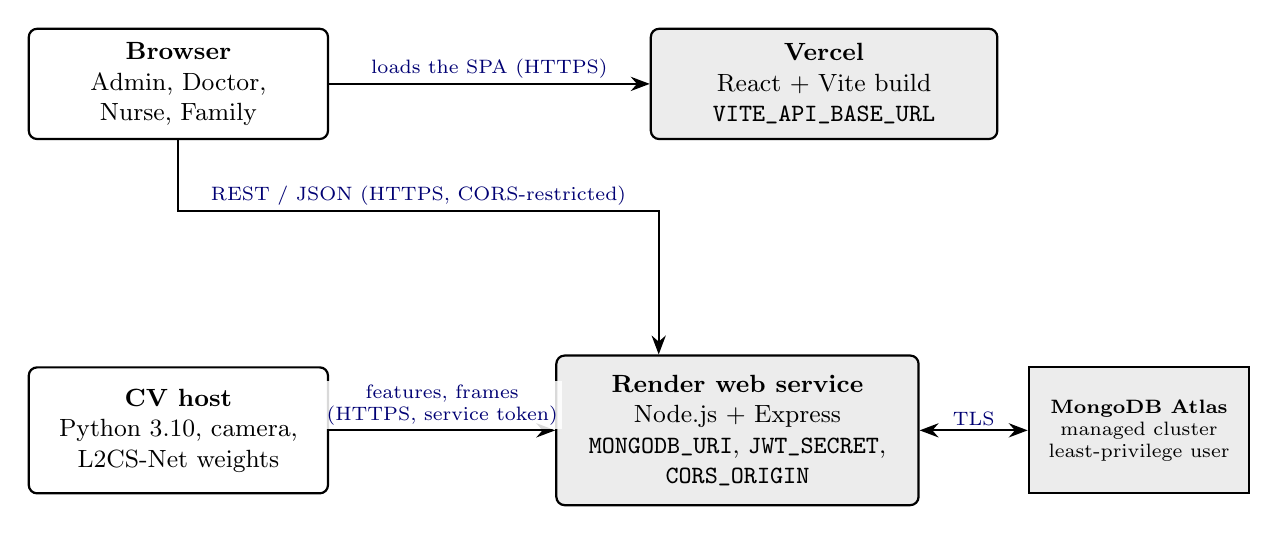
\begin{tikzpicture}[x=1cm,y=1cm, every node/.style={font=\scriptsize}]
  \node[box, minimum width=3.8cm, minimum height=1.4cm] (br) at (2.0,4.4) {\textbf{Browser}\\Admin, Doctor,\\Nurse, Family};
  \node[gbox, minimum width=4.4cm, minimum height=1.4cm] (ve) at (10.2,4.4) {\textbf{Vercel}\\React + Vite build\\\code{VITE_API_BASE_URL}};
  \node[box, minimum width=3.8cm, minimum height=1.6cm] (cv) at (2.0,0) {\textbf{CV host}\\Python 3.10, camera,\\L2CS-Net weights};
  \node[gbox, minimum width=4.6cm, minimum height=1.9cm] (re) at (9.1,0) {\textbf{Render web service}\\Node.js + Express\\\code{MONGODB_URI}, \code{JWT_SECRET},\\\code{CORS_ORIGIN}};
  \node[store, minimum width=2.8cm, minimum height=1.6cm] (at) at (14.2,0) {\textbf{MongoDB Atlas}\\managed cluster\\least-privilege user};
  \draw[arr] (br) -- node[lbl,above]{loads the SPA (HTTPS)} (ve);
  \draw[arr] (br.south) -- ++(0,-0.9) -| node[lbl,above,pos=0.25]{REST / JSON (HTTPS, CORS-restricted)} ([xshift=-1.0cm]re.north);
  \draw[arr] (cv) -- node[lbl,above,align=center]{features, frames\\(HTTPS, service token)} (re);
  \draw[darr] (re) -- node[lbl,above]{TLS} (at);
\end{tikzpicture}
\caption{Deployment view.}
\label{fig:deploy}
\end{figure}

\begin{longtable}{@{}>{\ttfamily\footnotesize}p{4.4cm}>{\raggedright\arraybackslash}p{2.6cm}>{\raggedright\arraybackslash}p{7.6cm}@{}}
\caption{Main configuration values}\\
\toprule \textbf{Variable} & \textbf{Component} & \textbf{Purpose}\\ \midrule \endfirsthead
\toprule \textbf{Variable} & \textbf{Component} & \textbf{Purpose}\\ \midrule \endhead
\bottomrule \endfoot
VITE_API_BASE_URL & Frontend & Base URL of the backend API.\\
MONGODB_URI & Backend & Atlas connection string (secret).\\
JWT_SECRET & Backend & Signing secret for user tokens (secret).\\
CORS_ORIGIN & Backend & Allowed frontend origin.\\
CV_SERVICE_TOKEN & Backend & Accepted service token for ingestion (secret; stored hashed).\\
STALE_AFTER_S, OFFLINE_AFTER_S & Backend & Freshness thresholds (default 5 s and 30 s).\\
SNAPSHOT_INTERVAL_S, SNAPSHOT_TTL_DAYS & Backend & History rate and expiry (default 1 s and 30 days).\\
ALERT_COOLDOWN_S & Backend & Alert suppression window (default 60 s).\\
BACKEND_URL, SERVICE_TOKEN, ENABLE_BACKEND & CV Service & Target API, token and on/off switch of the sender.\\
SEND_RATE_HZ, CAMERA_INDEX & CV Service & Post rate (default 2) and camera device.\\
\end{longtable}

\section{Legal, Ethical and Regulatory Conditions}
\begin{itemize}
  \item Any use of the system with real patients or volunteers needs approval from the responsible ethics body, informed consent, and a data-handling plan (A-07, NFR-PRV-05).
  \item The project does not claim regulatory approval or compliance (FR-LAND-04, NFR-PRV-07).
  \item Third-party components keep their licences: MediaPipe, OpenCV, PyTorch and the L2CS-Net weights and code used by the pipeline. The licence of the weights file shall be checked before redistribution.
\end{itemize}

\section{Documentation Deliverables}
Technical documentation, architecture diagrams, the OpenAPI description, a test report, screenshots and a demonstration of the complete monitoring workflow shall be delivered together with the source code and the final project report. The report shall say what is implemented, what is a heuristic, what is planned and what is not validated.

\section{Maintenance and Future Scope}
Likely extensions (not part of Version 1.0): secure real-time video streaming; additional sensors for multimodal fusion; improved temporal modelling and use of the trained model that already exists in the repository; clinician-annotated datasets for validation; alert rules that can be edited in the interface; better buffering and monitoring of the sender; role-specific accessibility work.

\section{Known Issues and Risks}\label{sec:risks}
The items below come from the static review of the repository and from the project proposal. They are risks to integration, not defects of this specification.

\begin{longtable}{@{}>{\ttfamily\footnotesize}p{1.1cm}>{\raggedright\arraybackslash}p{7.3cm}>{\raggedright\arraybackslash}p{6.2cm}@{}}
\caption{Known issues and risks}\label{tab:risks}\\
\toprule \textbf{ID} & \textbf{Issue or risk} & \textbf{Handled by}\\ \midrule \endfirsthead
\toprule \textbf{ID} & \textbf{Issue or risk} & \textbf{Handled by}\\ \midrule \endhead
\bottomrule \endfoot
R-01 & The sender posts to \code{/api/face-eye/features} and \code{/api/stream/face}; the in-repo FastAPI service defines only \code{/face}, \code{/posture} and \code{/fusion}, so the two do not match. & CVI-01, FR-ING-01\\ \midrule
R-02 & The sender is disabled by default, does not check HTTP status and has no retry; failures are silent. & CVI-04, CVI-06\\ \midrule
R-03 & The 1 s synchronous send inside the camera loop can stall inference. & CVI-03, NFR-PERF-02, NFR-PERF-06\\ \midrule
R-04 & The payload omits AUs, head pose, PERCLOS and gaze speed that the proposal's dashboard shows. & CVI-02, FR-LIVE-10\\ \midrule
R-05 & No heartbeat: ``no face in view'' cannot be told from ``CV Service stopped''. & CVI-06, FR-LIVE-13\\ \midrule
R-06 & The in-repo backend keeps only the latest values in RAM, has no history, no authentication and no frame route. & Replaced by this platform\\ \midrule
R-07 & An earlier frontend showed incorrect data and its cause was not recorded; its source is not in the repository. & NFR-TST-03 (contract test)\\ \midrule
R-08 & Comments and default values of the AU calibration in \code{config/settings.py} appear inconsistent (for example the AU6 range). & Audit with neutral-face logs before AU values are shown as results\\ \midrule
R-09 & Gaze durations assume 30 FPS; the saccade window comment (150 frames) differs from its description; gaze angles are in radians. & CVI-09, FR-ING-14\\ \midrule
R-10 & In the eye-closed branch the gaze tracker returns zeroed variance and speed fields. & FR-LIVE-07\\ \midrule
R-11 & The JSONL log lacks gaze and behaviour state; the CSV is overwritten at each run while the JSONL is appended. & CVI-11; note for experiments\\ \midrule
R-12 & Root \code{requirements.txt} and \code{requirements/} differ (CUDA pins, duplicate OpenCV packages); the README mentions an \code{L2CS-Net} folder that does not exist. & One tested install path per target (Windows, Jetson, Docker)\\ \midrule
R-13 & The indices are not clinically validated; a trained XGBoost model exists but \code{main.py} does not use it. & BR-01, BR-02, BR-09\\ \midrule
R-14 & Free-tier hosting limits (idle spin-down, storage, no GPU). & C-04, C-12, DR-05\\ \midrule
R-15 & Camera and patient data are sensitive. & NFR-PRV-01 to NFR-PRV-07\\ \midrule
R-16 & The pipeline was reviewed statically and has not been run end-to-end against the platform. & A-01; integration tests NFR-TST-05\\
\end{longtable}

\appendix
\chapter{Traceability Matrix}\label{app:trace}
\begin{longtable}{@{}>{\raggedright\arraybackslash}p{1.1cm}>{\raggedright\arraybackslash}p{5.0cm}>{\raggedright\arraybackslash}p{4.4cm}>{\raggedright\arraybackslash}p{3.6cm}@{}}
\caption{Objectives, proposal objectives, requirements and verification}\\
\toprule \textbf{Obj.} & \textbf{Objective (Section 1.5)} & \textbf{Requirements} & \textbf{Proposal obj. / verification}\\ \midrule \endfirsthead
\toprule \textbf{Obj.} & \textbf{Objective} & \textbf{Requirements} & \textbf{Proposal obj. / verification}\\ \midrule \endhead
\bottomrule \endfoot
O1 & Integrate the existing pipeline through a versioned contract & FR-ING, CVI, Table~\ref{tab:payload} & 1, 5 / NFR-TST-03, -05\\ \midrule
O2 & Secure role-based access & FR-AUTH, FR-WS, NFR-SEC & 7 / NFR-TST-02, -06\\ \midrule
O3 & Persist data in MongoDB Atlas & DR-01 to DR-08, FR-PAT, FR-SESS & 6 / NFR-TST-01, -05\\ \midrule
O4 & Live view with explicit stale and missing states & FR-LIVE, FR-ING-07, NFR-PERF-01, NFR-REL-03 & 8 / NFR-TST-05, -07\\ \midrule
O5 & Events and alerts with acknowledgement & FR-EVT & 9 / NFR-TST-01, -06\\ \midrule
O6 & Historical charts and summaries & FR-HIST, FR-ING-08 & 9 / NFR-TST-02\\ \midrule
O7 & Rooms, shifts, tasks, medication records & FR-ADM, FR-NUR, FR-DOC & 9 / NFR-TST-02, -06\\ \midrule
O8 & Responsive interface modelled on the reference video & Section 2.8, IR-UI, NFR-USE & 2, 3 / NFR-TST-06\\ \midrule
O9 & Deployment on Vercel, Render and Atlas & Section 5.1, C-01 to C-04 & 4, 10 / deployment test\\ \midrule
O10 & Testing and documentation without clinical claims & Chapter 4, BR, Section 5.3 & 11, 12 / NFR-TST-08\\
\end{longtable}

\chapter{Example Payload}\label{app:json}
The listing shows the shape of a version~1.1 payload. All values are illustrative only and are not measurements.
\begin{lstlisting}[basicstyle=\ttfamily\scriptsize, breaklines=true, frame=single, columns=fullflexible]
{
  "schema_version": "1.1",
  "units": { "gaze": "rad", "head_pose": "deg" },
  "patient_id": "P001",
  "timestamp_unix": 1760000000.123,
  "behavior_state": "alert",
  "global_distress": 12.0,
  "pain_index": 8.0, "fear_index": 5.0, "fatigue_index": 20.0,
  "agitation_index": 3.0, "tension_index": 10.0, "respiratory_index": 4.0,
  "gaze_yaw": 0.05, "gaze_pitch": -0.02, "gaze_variance": 0.01,
  "fixation_duration": 0.8, "recent_saccades": 2, "eye_contact_ratio": 0.7,
  "episode_pain": false, "episode_agitation": false, "episode_fatigue": false,
  "episode_fear": false, "episode_eye_closure": false,
  "face_confidence": 0.9,
  "baseline_ready": true, "fps": 24.5, "pipeline_version": "5405f41",
  "head_pose": { "yaw": 3.0, "pitch": -2.0, "roll": 1.0 },
  "perclos": 0.1
}
\end{lstlisting}

\chapter{Reference User-Interface Screens}\label{app:ui}
The figures are frames taken from the supplied reference video. They show the layout and navigation that the new interface follows; the content shown in them (vitals, posture, audio, risk predictions, sample names and numbers) is not part of this system's data.

\begin{figure}[h!]
\centering
\begin{tabular}{@{}cc@{}}
\includegraphics[width=0.485\textwidth]{figures/ui_landing.jpg} & \includegraphics[width=0.485\textwidth]{figures/ui_workspace.jpg}\\
\small (a) Landing page & \small (b) Select Your Workspace\\[4pt]
\includegraphics[width=0.485\textwidth]{figures/ui_doctor.jpg} & \includegraphics[width=0.485\textwidth]{figures/ui_live_monitor.jpg}\\
\small (c) Doctor dashboard & \small (d) Live Patient Monitor\\[4pt]
\includegraphics[width=0.485\textwidth]{figures/ui_medication.jpg} & \includegraphics[width=0.485\textwidth]{figures/ui_admin_rooms.jpg}\\
\small (e) Nurse medication schedule & \small (f) Admin room management\\
\end{tabular}
\caption{Reference screens from the supplied video.}
\label{fig:refui}
\end{figure}

\chapter{Open Decisions}\label{app:open}
\begin{idtable}{Decisions to confirm with the supervisor and team}
\idr{D-01}{Final role set and whether the Family workspace belongs in Version 1.0.}
\idr{D-02}{Where the CV Service runs (laboratory PC, Jetson device or cloud GPU) and how its token is provisioned.}
\idr{D-03}{Retention periods for snapshots, events and clinical records, and the ethics approval needed.}
\idr{D-04}{Polling or Server-Sent Events/WebSockets for the live view, based on the measured latency.}
\idr{D-05}{Alert thresholds and cool-down values, and who may change them.}
\idr{D-06}{Token delivery (HttpOnly cookie or bearer header) and the idle time-out.}
\idr{D-07}{Whether live preview video is required for the demonstration, and the bandwidth limit.}
\idr{D-08}{Size of the seeded room and floor data (the reference video shows five floors of 40 rooms).}
\idr{D-09}{JavaScript or TypeScript for frontend and backend.}
\idr{D-10}{Annotated dataset and metrics for any evaluation of CV accuracy; this is separate from the website integration.}
\end{idtable}
\end{document}